%!TEX TS-program = pdflatex
%!TEX root = i3det-top.tex
%!TEX encoding = UTF-8 Unicode

\section{\label{sect:online}Online Systems}

The IceCube online systems comprise both the software and hardware at the
detector site responsible for data acquisition, event selection,
monitoring, and data storage and movement.  As one of the goals of IceCube
operations is to maximize the fraction of time the detector is sensitive to
neutrino interactions (``uptime''), the online systems are modular so that
failures in one particular component do not necessarily prevent the
continuation of basic data acquisition. Additionally, all systems are
monitored with a combination of custom-designed and industry-standard tools
so that detector operators can be alerted in case of abnormal conditions.

\subsection{\label{sect:online:dataflow}Data Flow Overview}

The online data flow consists of a number of steps of data reduction and
selection in the progression from photon detection in the ice to
candidate physics event selection, along with associated secondary
monitoring and data streams.  An overview of the data flow is shown in
Fig.~\ref{fig:online_dataflow}.

\begin{figure}[!ht]
 \centering
 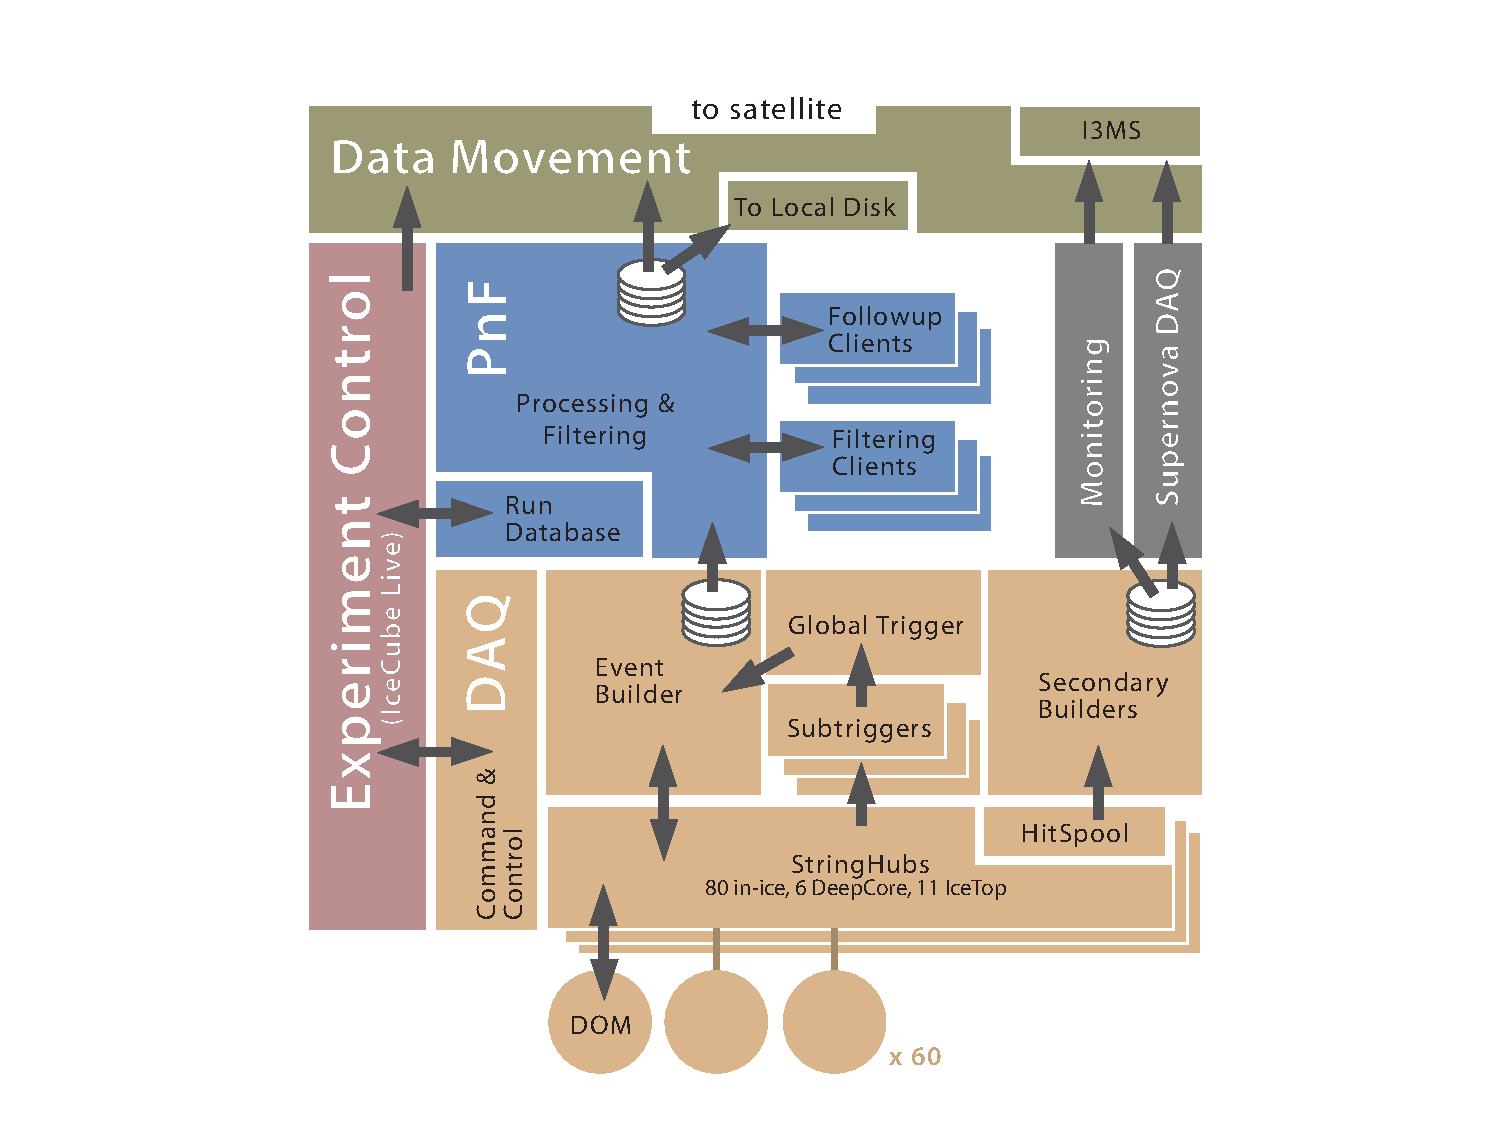
\includegraphics[width=0.6\textwidth]{graphics/online/online_dataflow.pdf}
 \caption{Data flow in the primary IceCube online systems. See details
   on each component in the text.}
 \label{fig:online_dataflow}
\end{figure}

DOM hits are mostly due to dark noise. The first step
in data reduction takes place in the DOM, using the Local Coincidence (LC) condition described in
Sec.~\ref{sec:dom_functional}.  Hits that meet the LC criteria are flagged
as Hard Local Coincidence (HLC hits) and include a full payload of
digitized waveforms, while isolated non-LC hits are flagged as Soft Local
Coincidence (SLC) hits and are compressed more aggressively, with only a
timestamp and minimal amplitude / charge information transmitted.

All DOM hits are read out to dedicated computers on the surface
(Sec.~\ref{sect:sps}) by the data acquisition system (DAQ).  The next level
of data selection is the formation of software triggers by the DAQ
system. HLC hits across the detector are examined 
for temporal and in some cases spatial patterns that suggest a common
causal relationship.  A number of different trigger algorithms run in
parallel, described in Sec.~\ref{sect:online:trigger}.  All hits (both HLC
and SLC) within a window around the trigger are combined into events, the
fundamental output of the DAQ.  The event rate varies
seasonally with the atmospheric muon flux~\cite{ICECUBE:IceTop} from 2.5 to
2.9 kHz, with a median rate of 2.7 kHz, and the total DAQ data rate is
approximately 1~TB/day. 

The DAQ also produces secondary streams that include time calibration,
monitoring, and DOM scaler data.  The scaler data, which monitors the
hit rate of each DOM, is used in the supernova data
acquisition system (Sec.~\ref{sect:SNDAQ}).  The time calibration and
monitoring streams are used to monitor the health and quality of the
data-taking runs.

The DAQ event data are then processed further with approximately 25 filters
in order to select a subset of events (about 15\%) to transfer over
satellite to the Northern Hemisphere (Sec.~\ref{sect:online:filter}).  Each
filter, typically designed to select events useful for a particular physics
analysis, is run over all events using a computing cluster in the ICL.
Because of limitations both on total computing power and bounds on the
processing time of each event, only fast directional and energy
reconstructions are used.  This Processing and Filtering (PnF) system is
also responsible for applying up-to-date calibration constants to the DAQ
data. All processed events, even those not selected by the online filters,
are archived locally.

A dedicated system for data movement, JADE, handles the local archival storage to
tape or disk and the handoff of satellite data
(Sec.~\ref{sect:online_jade}).  This includes not only primary data streams
but also monitoring data, calibration runs, and other data streams.
Low-latency communications for experiment control and real-time monitoring
are provided by the IceCube Messaging System (I3MS).  
Experiment control and detector monitoring are handled by the IceCube Live
software system, described in Sec.~\ref{sec:online:icecubelive}.

Data-taking runs are arbitrarily divided into 8-hour periods and assigned
a unique run number; data acquisition need not actually pause during
this transition.  Detector configuration parameters that affect physics
analyses are changed at most once per year (typically in May), indicating
the start of a new ``physics run''.   

\subsection{\label{sect:sps}South Pole System and South Pole Test System}

The South Pole System (SPS) comprises 19 racks of computing and network
hardware that run the various online systems described in this
section.  The DOM surface cables are connected via passive patch panels to
custom 4U computers, called DOMHubs, one DOMHub per in-ice string and 11 additional
hubs for IceTop.  The remaining servers, including those for higher-level
data acquisition, event filtering, detector monitoring, and core
infrastructure, are currently 2U Dell PowerEdge R720 servers running
Scientific Linux (Table \ref{tab:sps_breakdown}).  The servers are
typically upgraded every three to four years.  The custom hardware components in
the DOMHubs are replaced with spares as failures warrant, and the disks and
single-board computer were upgraded in 2013--14.

\begin{table}[h]
  \centering
\caption{Breakdown of computing equipment at SPS, indicating number of
    machines used for each task.}
  \begin{tabular}{ r  c }
\hline
    Component & \# \\ \hline DOMHubs & 97 \\ Other data
    acquisition & 4 \\
%    Experiment control & 1 \\
    Monitoring & 3 \\ Event filtering & 24 \\ System infrastructure & 8 \\ Other &
    6 \\
\hline
  \end{tabular}
  \label{tab:sps_breakdown}
\end{table}

The DOMHub is an industrial computer chassis with custom components for DOM
power, timing, and communication.  A low-power single-board computer
communicates with 8 custom PCI DOM Readout (DOR) cards via an
industry-standard backplane.  An ATX power supply with two
redundant modules powers the DOMHub, while two
48VDC Acopian power supplies, mounted and connected in series inside the
chassis to double the voltage to 96~V, supply power to the DOMs.  The DOM power is switched and
monitored by the DOR cards and is controlled by software.  Another PCI
card, the DOMHub Service Board (DSB), is responsible for GPS timing fanout
(Sec.~\ref{sect:online:master_clock}).

The SPS computers are connected via switches in each rack that provide
redundant connections to a 10--20 Gbps network backbone.  The DOMHubs are
connected to the rack switches with two bonded 1 Gbps links.  Typical network I/O during
data-taking for the DAQ Event Builder (Sec.~\ref{sect:online:evbuilder}) is about 240~Mbps in each direction.
The PnF Central Server sees 200 Mbps in and 640 Mbps out; the output
direction is significantly higher than the input as PnF distributes the
events to filtering clients and generates multiple output streams
(Sec.~\ref{sect:online:filter}).  

Redundancy and continuous monitoring of SPS is one of the keys to a high
detector livetime (Sec.~\ref{sec:operational_performance}).
Industry-standard Nagios monitoring software detects and flags problems, 
including issues with DOM power and communication on the DOMHubs.  Severe
problems impacting data-taking result in a page to the IceCube winterover 
personnel via the station's Land Mobile Radio (LMR) system.  A dedicated
powered spare server can replace any failed DAQ node, and spare PnF filtering
clients can be started to increase throughput in case of a data filtering
backlog.  SPS hardware is also connected to uninterruptible
power supplies (UPS) in order to continue data-taking through station power
outages of up to 15 minutes.

Total power usage of the detector and online systems, including computing servers, is
approximately 53 kW.  The majority is consumed by the DOMs, with an
average power consumption of 5.7W each, including power supply efficiency
and transmission losses, for a total of 30.6 kW.  The DOMHubs require 128W
each not including the DOM power, for a total of 12.4 kW.  The
computing servers consume approximately 200--300W each, depending on
configuration.  Most of the of the remaining power is used by the PnF
Filter Clients: 20 servers of 300W each for a total of 6 kW.

A scaled-down version of SPS, the South Pole Test System (SPTS) located in
Madison, Wisconsin, U.S.A., allows testing and validation of both hardware
and software in the Northern Hemisphere before rollout to SPS.  Servers and DOMHubs
identical to those at SPS, along with a small number of DOMs in chest
freezers, are used in the test system.  Although the number of DOMs
available is much smaller than in the real detector, recent software
improvements allow the ``replay'' of pre-recorded raw SPS hit data
on SPTS systems, providing a data stream to higher-level DAQ and PnF
components identical to SPS.  Another test system includes a full-length
in-ice cable and is used primarily for validation of DOM communications and
timing.

\subsection{Data Readout and Timing}

While the low-level communications and timing systems of the DOM are
described in detail in Ref.~\cite{ICECUBE:DAQ}, we review those here in
the broader context of the online systems.

\subsubsection{\label{sect:online:comms}Communications}

Digital communication between the DOR card and DOM occurs via copper
twisted pairs, with two DOMs per pair on the in-ice cable, and one IceTop
DOM per pair for increased bandwidth (IceTop hit rates can exceed 3 kHz).
The physical layer signaling uses on-off keying with bipolar pulses.  The
protocol is a custom 
packet-based scheme.  Each packet is assigned a sequence number, and all
received packets are acknowledged if the sequence number is correct.  Each
packet also contains a cyclic redundancy checksum to detect transmission errors.
Out-of-sequence packets received are ignored, and non-acknowledged packets
are retransmitted. The total bandwidth of the communication channel
is 720 kbps per twisted pair.

Messaging is managed from the surface, in that the DOR requests data from
each DOM in turn; only one DOM per pair can transmit at a time.  Communication is
paused once per second to perform a timing calibration (RAPCal; Sec.~\ref{sect:dom:rapcal}); this enables time transfer of DOM clock to DOR
clock for every DOM.  

% Add more details about actual usage?
% Q: is LC signaling documented anywhere yet?  Should it go here?

\subsubsection{\label{sect:online:master_clock}Master Clock System}

The DOR clocks themselves are synchronized to UTC via an active fanout
system from a single Symmetricom ET6000 GPS receiver with a
temperature-stabilized 10 MHz oscillator, also known as the Master
Clock. The fanout tree is shown in
Fig.~\ref{fig:clock_fanout}. The 10 MHz output, a 1 Hz output, and a
proprietary serial time string indicating
the UTC date and time are distributed to the DOMHubs via a series of
fanouts, using shielded, delay-matched twisted-pair cables.  Within the
DOMHub, the DSB card continues the fanout via short delay-matched patch
cables to each DOR card.  The local 20 MHz clocks of each DOR card are
phase-locked to the distributed 10 MHz signal.  

To avoid the Master Clock being a single-point failure for the detector, a
hot spare receiver, using its own GPS antenna and powered through a
dedicated UPS, is continuously active and satellite-locked in case of problems with
the primary.

\begin{figure}[!ht]
 \centering
 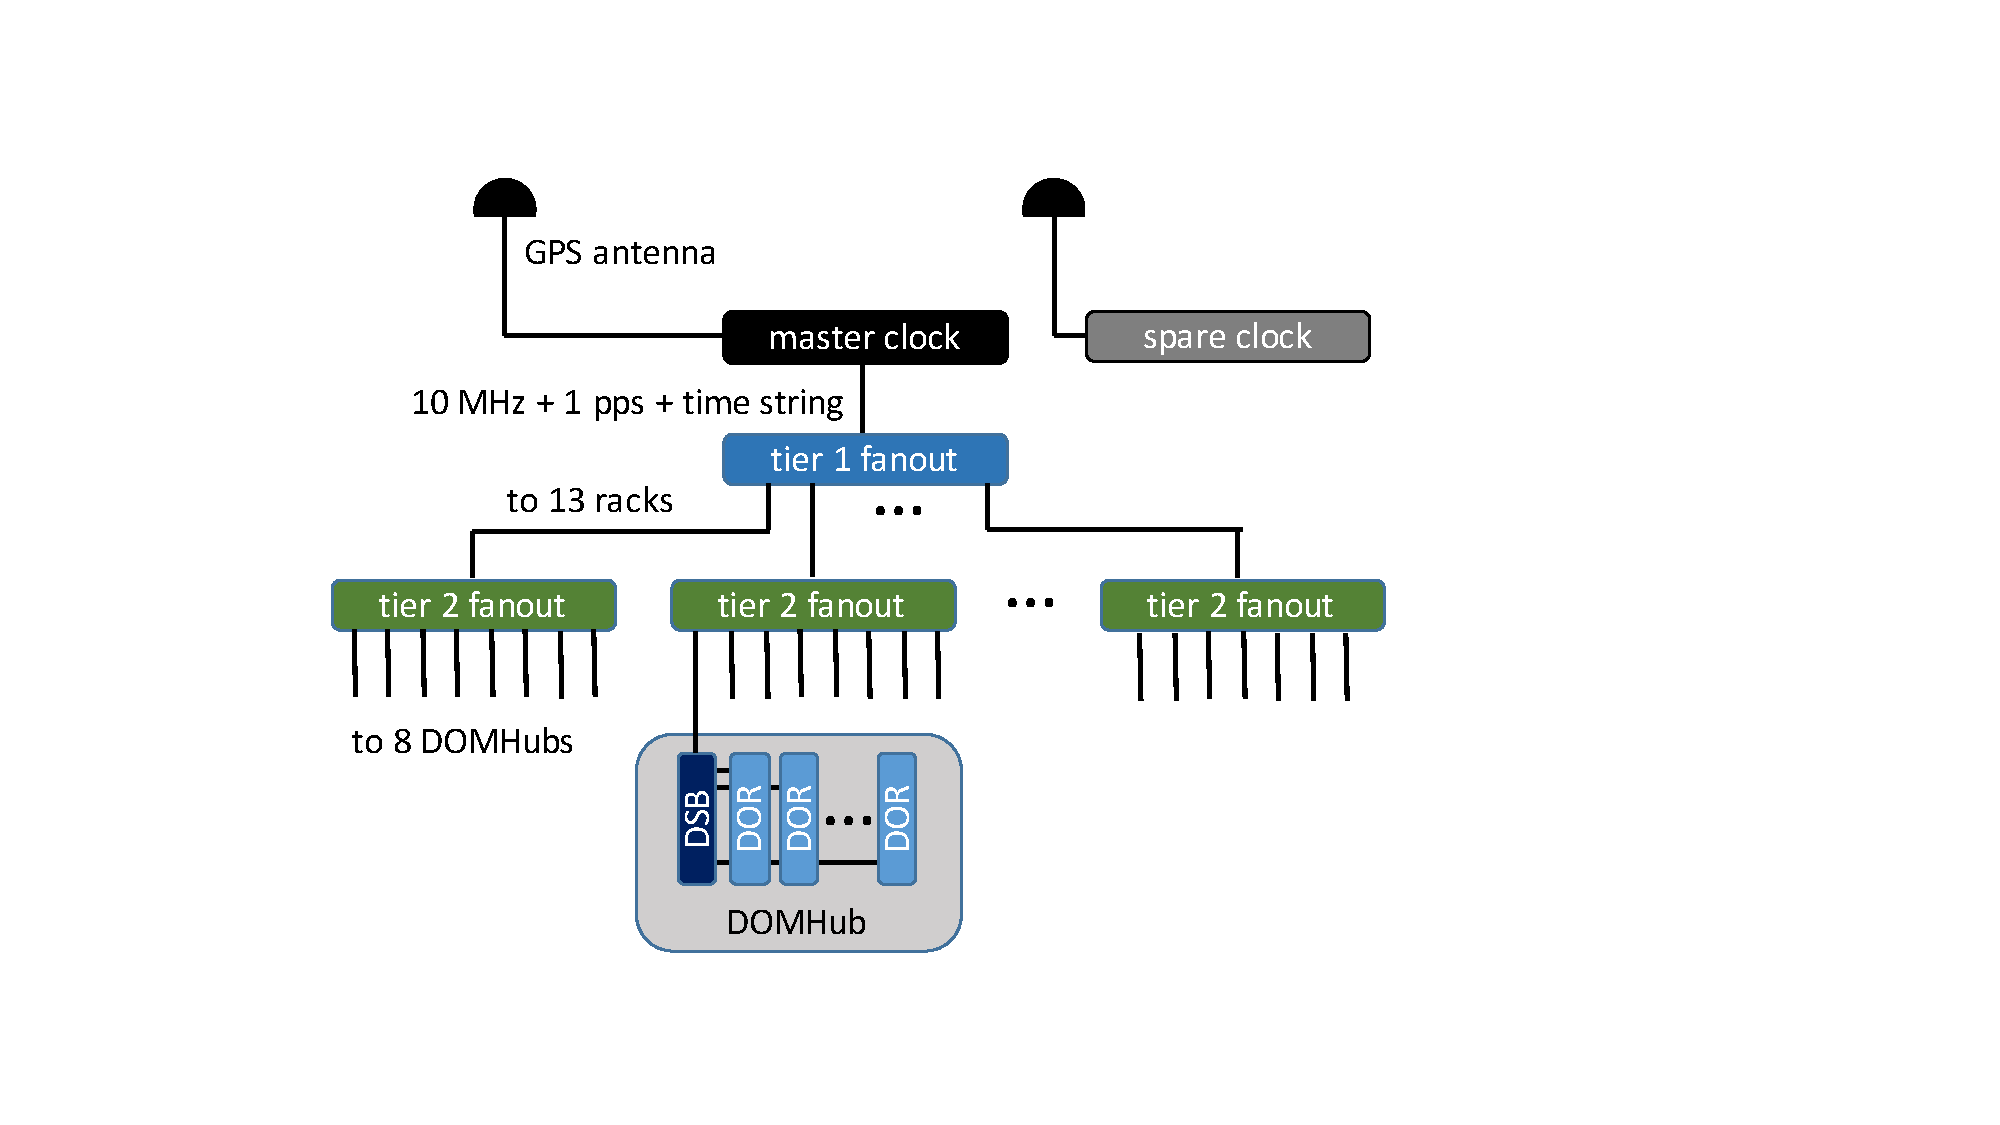
\includegraphics[width=0.8\textwidth]{graphics/online/data_readout/clock_fanout.pdf}
 \caption{Master Clock fanout system, from GPS receiver to DOR cards in
   each DOMHub.}
 \label{fig:clock_fanout}
\end{figure}

% Q: do we correct for fanout delay of ~150 ns anywhere?
% Q: say anything about leap seconds?

\subsubsection{DOR Card and Driver}

Each DOR card is connected to up to 8 DOMs, with 8 DOR cards in a
DOMHub. The DOR card controls the 96~VDC power supply to the DOMs and
modulates the communications signaling on top of this DC level; the DOMs
can accept input voltages from 40--120 V.
Dedicated circuitry monitors the current draw and voltage levels on each
twisted pair. A ``firmware fuse'' can disable power if the current draw
deviates from programmable maximum or minimum levels, and this mechanism is
supplemented with standard physical fuses.  

The software interface to the DOR card, and thus to the DOMs, is provided
with a custom Linux device driver.  Access to DOR card functions, including
DOM power control, communication statistics, RAPCal, and current / voltage
monitoring, is facilitated using the Linux \texttt{/proc} filesystem
interface.  Data transfer from the cards to the single-board computer is
achieved via Direct Memory Access (DMA) over the PCI bus.  The driver
provides a device file for each DOM for read/write access by higher-level software.

\subsection{Data Acquisition Software}

IceCube's data acquisition (DAQ) system is a set of software components
running on the DOMHubs and dedicated servers in the ICL.  These components are shown in
Fig.~\ref{fig:online_dataflow} and include StringHub, Trigger, Event
Builder, Secondary Builder, and a Command and Control server.  The DAQ is
responsible for detecting patterns of hits in the detector likely to be
caused by particle interactions and storing these collections of hits as
``events''.

Hits are read continuously from the DOMs by the
StringHub components running on each DOMHub, and a minimal representation of each HLC hit is
forwarded to the Subtrigger components (either the in-ice or IceTop Subtrigger.)
The Subtrigger components apply a
configurable set of algorithms to the hit stream and form windows around interesting temporal
and/or spatial patterns.  These time windows are collected by the
Global Trigger and used to form non-overlapping trigger requests by merging
subtriggers as needed, ensuring that the same hit doesn't appear in
multiple events.  The merged trigger requests are used by the Event Builder
component as templates 
to gather the complete hit data from each StringHub and assemble the final
events.

\subsubsection{StringHub and HitSpool}
\label{sec:domhub_hitspool}

The StringHub software component that runs on each DOMHub is responsible
for reading all available data from each of its connected DOMs each second
and passing that data onto the downstream consumers.  It also saves all
hits to a local ``HitSpool'' on-disk cache and queues them in an
in-memory cache to service future requests from the Event Builder for full
waveform data.

The StringHub component is divided into two logical pieces: the front
end is called Omicron and the back end is the Sender. Omicron controls all
of the connected DOMs, forwarding any 
non-physics data (calibration, monitoring) to its downstream consumers and
sorting the hits from all 
DOMs into a single time-ordered stream before passing them to the Sender.  

Omicron is also responsible for translating DOM hit times into
UTC-compatible ``DAQ time'', which counts the number of 0.1-ns periods
since the UTC start of the year (including leap seconds).  The translation
uses the RAPCal procedure as described in Sec.~\ref{sect:dom:rapcal},
performed for each DOM every second.  

The Sender caches SLC and HLC hits in memory, then forwards a
condensed version of each HLC hit to the appropriate local Trigger. Each
condensed HLC hit record contains the hit time, a DOM identifier, and the
trigger mode.  After the
Trigger components have determined interesting time intervals, 
the Event Builder requests each interval from the Sender which returns a list of
all hits within the interval and prunes all older hits from the in-memory hit
cache after each interval.

One core requirement of the DAQ is that each component operates on a
time-ordered stream of data.  The DAQ uses its ``Splicer'' to accomplish
this.  The Splicer is an object that gathers all input streams
during the setup phase at the beginning of a data-taking run; no inputs can
be added once started.  Each stream 
pushes new data onto a ``tail'', and the Splicer merges the data from all
streams into a single sorted output stream.  When a stream is closed, it
issues an end-of-stream marker that causes the Splicer to
ignore all further data.  Details of the Splicer algorithm can be found in
Ref.~\cite{vlvnt13_trigger}.  

As hits move from Omicron to the Sender, they are written to the
HitSpool disk cache.  These files are
written in a circular order so that the newest hits overwrite the oldest
data.  The files are catalogued in a SQLite database to
aid in fast retrieval of raw hit data.

One limitation of the current design is that it only reads data when
the full DAQ system is running, so the detector is essentially ``off''
during certain hardware failures or the periodic full restarts of the
system that occur every 32 hours.  A future enhancement 
will split the StringHub into several independent pieces to eliminate these
brief pauses.  The front end (Omicron) will be moved to a daemon
that continuously writes data (including secondary, non-physics data and
other metadata) to the disk cache.  Part of the back end (Sender) 
will become a simple HitSpool client that reads data from the disk cache
and sends it to the downstream consumers, while another simple component
will listen for requested hit readout time intervals from the Event Builder
and return lists of hits taken from the HitSpool.

\subsubsection{\label{sect:online:trigger}Triggers}

The DAQ trigger algorithms look for clusters of HLC hits in space and time
that could indicate light due to a particle interaction in the detector, as
opposed to uncorrelated dark noise.   An algorithm searches for a given
multiplicity of HLC hits, possibly with an additional geometric
requirement, within a trigger time window.  The time scale of the trigger window is
set by the light travel time in ice and the geometry requirement
involved. Longer readout windows are appended before and after the trigger
windows to save early and late hits with the events.

Triggers are generally restricted to a subset of DOMs, such as all in-ice DOMs,
IceTop DOMs, or DeepCore DOMs.  The algorithms run in parallel over all
hits in the DOM set, and then overlapping triggers are merged.  The various
trigger algorithms are described below, and a summary of the algorithm
parameter settings is found in Table \ref{tab:triggers}.  Trigger settings
are changed at most once per year.

The fundamental trigger for IceCube, IceTop, and DeepCore is the Simple
Multiplicity Trigger (SMT).  The SMT requires $N$ or more HLC hits within a
sliding time window of several $\mu\mathrm{s}$, without any locality
conditions.  Once the multiplicity condition is met, the trigger is 
extended until there is a time period of the length of the initial trigger
window without any HLC hits from the relevant DOM set.  The
multiplicity value $N$ is tuned to the energy threshold of the sub-detector,
which fundamentally is set by the string or tank spacing.

Other triggers use a lower multiplicity threshold by adding constrains on
the HLC hit topology.  The time windows for these triggers are based upon
the size of the locality volume. The Volume Trigger defines a cylinder of fixed size around
each hit DOM and requires a given multiplicity within this cylinder
(Fig.~\ref{fig:trig_cylinder}); this allows one to trigger on localized
low-energy events that do not satisfy the SMT condition.  The Volume Trigger
has an additional simple multiplicity parameter that fires the trigger when
a certain number of hits is reached, regardless of any spatial
restrictions; this prevents the trigger 
algorithm from slowing down when the detector has triggered already from
the primary SMT. The String Trigger requires a certain number of hits
within a span of DOMs along a single string 
(Fig.~\ref{fig:trig_string}); this allows one to trigger on low-energy
muons that pass vertically through the detector.

\begin{figure}[ht]
  \centering \subfloat[]{
    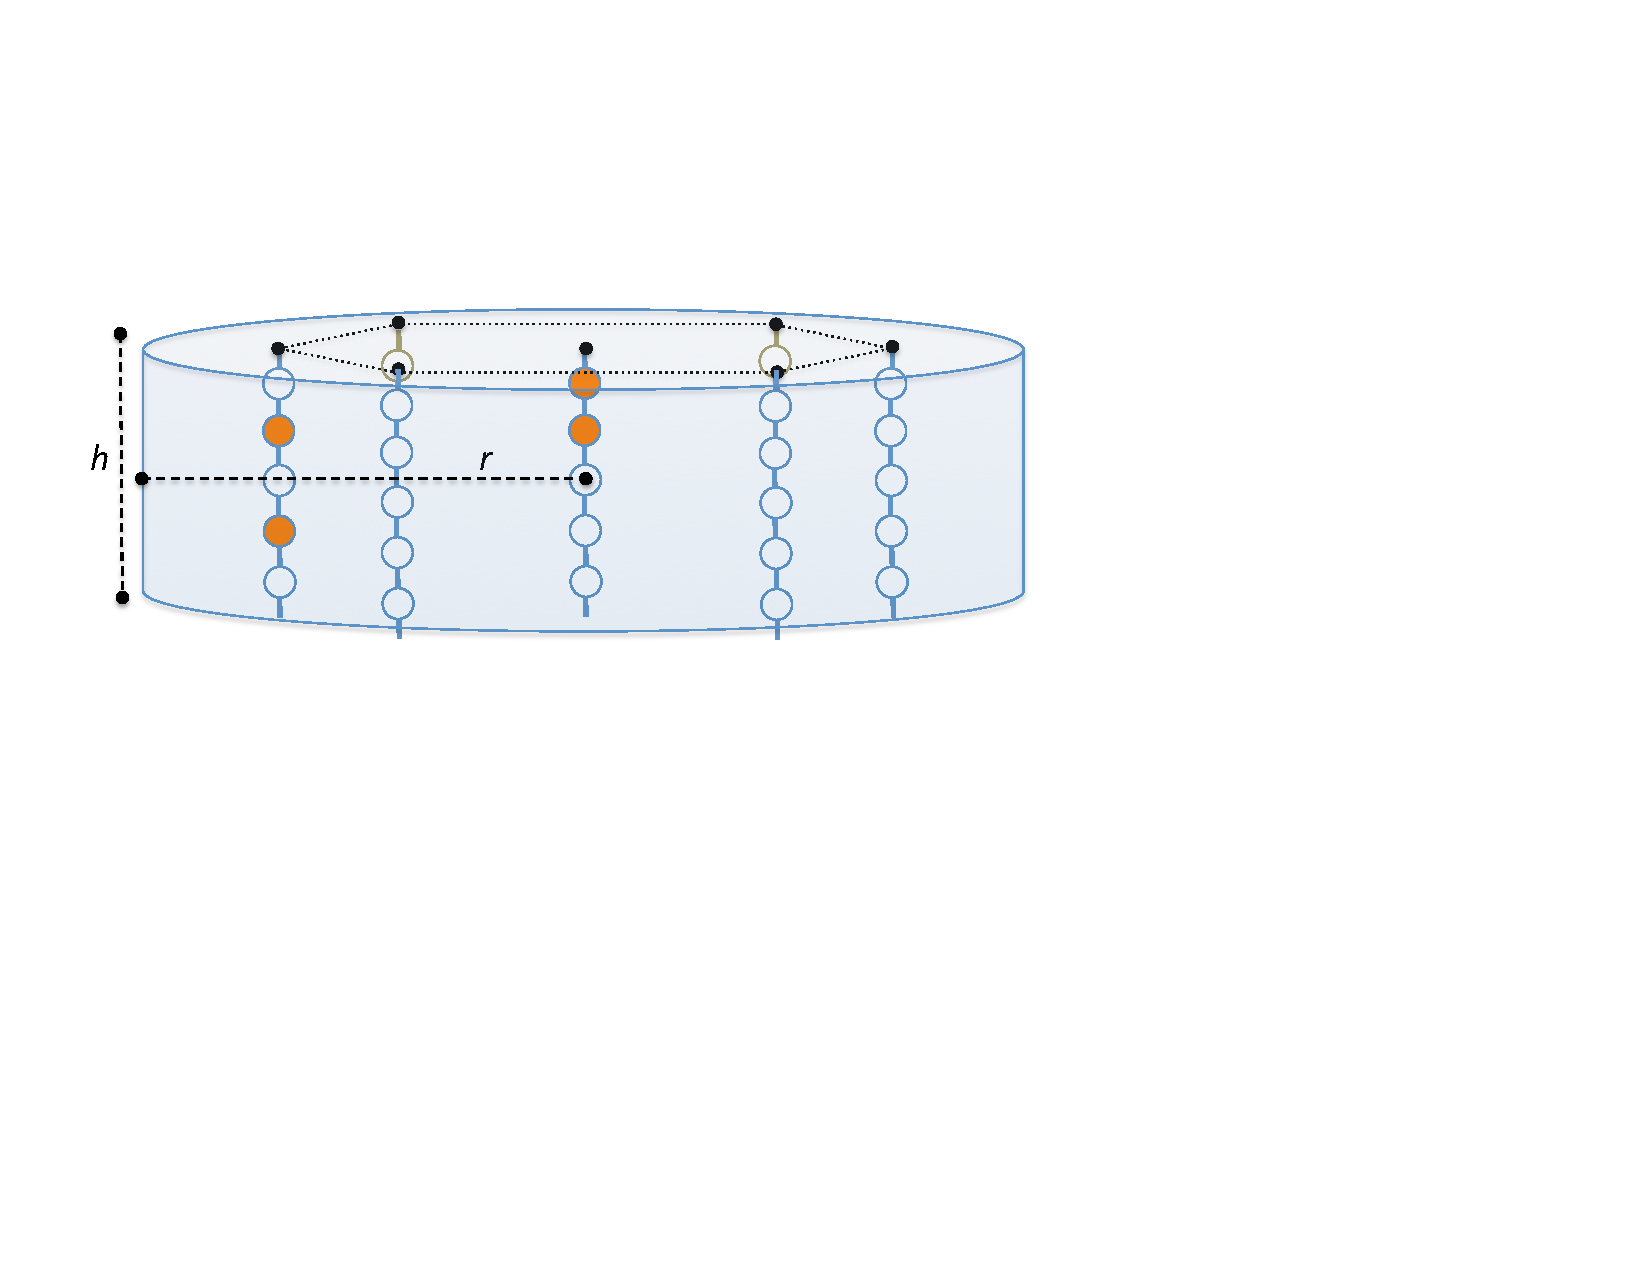
\includegraphics[scale=0.45]{graphics/online/trigger/trig_cylinder}
    \label{fig:trig_cylinder}
  }
  \quad
  \subfloat[]{
    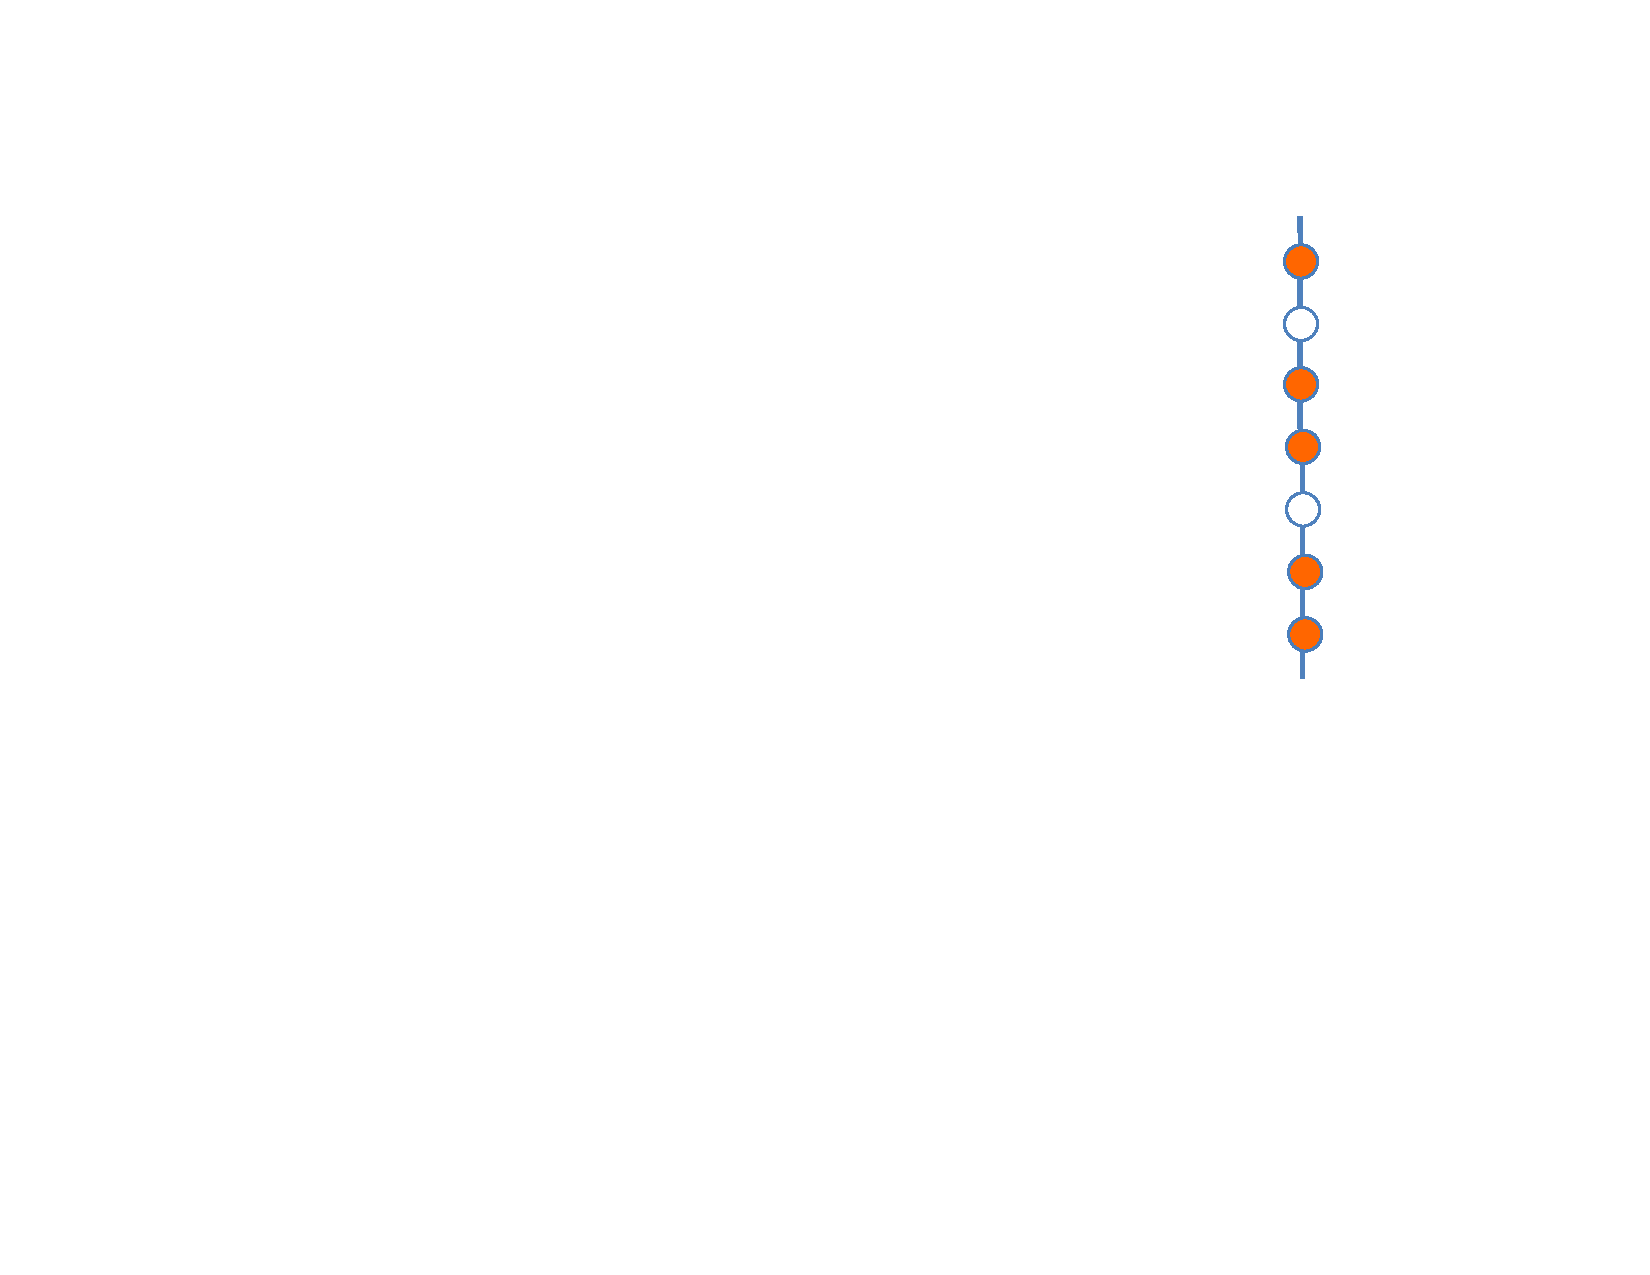
\includegraphics[scale=0.5]{graphics/online/trigger/trig_string}
    \label{fig:trig_string}
  }
  \caption{Schematic representation of triggers using spatial coincidences.  Shaded circles
    represent HLC-hit DOMs.  Left: Volume Trigger.  Right: String Trigger. }
\end{figure}

IceCube has the potential to detect hypothetical subrelativistic heavy
particles such as magnetic monopoles via catalyzed nucleon decays along
the particle trajectory \cite{Aartsen:2014awd}.  However, because these
particles may travel at velocities less than $0.01c$, the time
windows used in the standard triggers are too short.  A dedicated Slow
Particle (SLOP) trigger has thus been developed to search for slow
track-like particle signatures.

The SLOP trigger operates in several stages.  The HLC hits, which by design
come in at least in pairs along a string, are cleaned by removing pairs that
are proximate in time ($\Delta t < T_{\mathrm{prox}}$); $T_{\mathrm{prox}}$
is tuned to remove most hits from particles traveling near $c$, such as muons.
For all parameters, the trigger algorithm considers the time and 
position of the first hit within each HLC pair.  Next, triplets of HLC
pairs within a time window $T_{\mathrm{max}}$ 
are formed.  The geometry of each triplet formed (Fig.~\ref{fig:slop})
must satisfy track-like 
conditions: the largest inner angle $\alpha$ of the triangle formed by the
HLC pairs must be greater than $\alpha_{\mathrm{min}}$, and the
``velocities'' along the triangle sides must be consistent.  Specifically,
the normalized inverted velocity difference $v_\mathrm{rel}$, defined as

\begin{equation}
  v_\mathrm{rel}=\frac{|\Delta
  v_\mathrm{inverse}|}{\overline{v}_\mathrm{inverse}} = 
  3\cdot\frac{|\frac{1}{v_{23}}-\frac{1}{v_{12}}|}
  {\frac{1}{v_{12}}+\frac{1}{v_{23}}+\frac{1}{v_{13}}}
%  v_{\mathrm{rel}} = 3\left|\frac{1}{v_{12}} - \frac{1}{v_{23}}\right|/\left(\frac{1}{v_{12}} +
%  \frac{1}{v_{23}} + \frac{1}{v_{13}}\right)
\end{equation}

\noindent where $\ v_{ij} = \Delta x_{ij}/\Delta t_{ij}$, must be less than
or equal to a predefined maximum value
$v_{\mathrm{rel}}^{\mathrm{max}}$.  Finally, the total number of track-like triplets
must be greater than or equal to $N_{\mathrm{triplet}}$, set to 5, and all
of these track-like triplets must overlap in time.  

\begin{figure}[!ht]
 \centering
 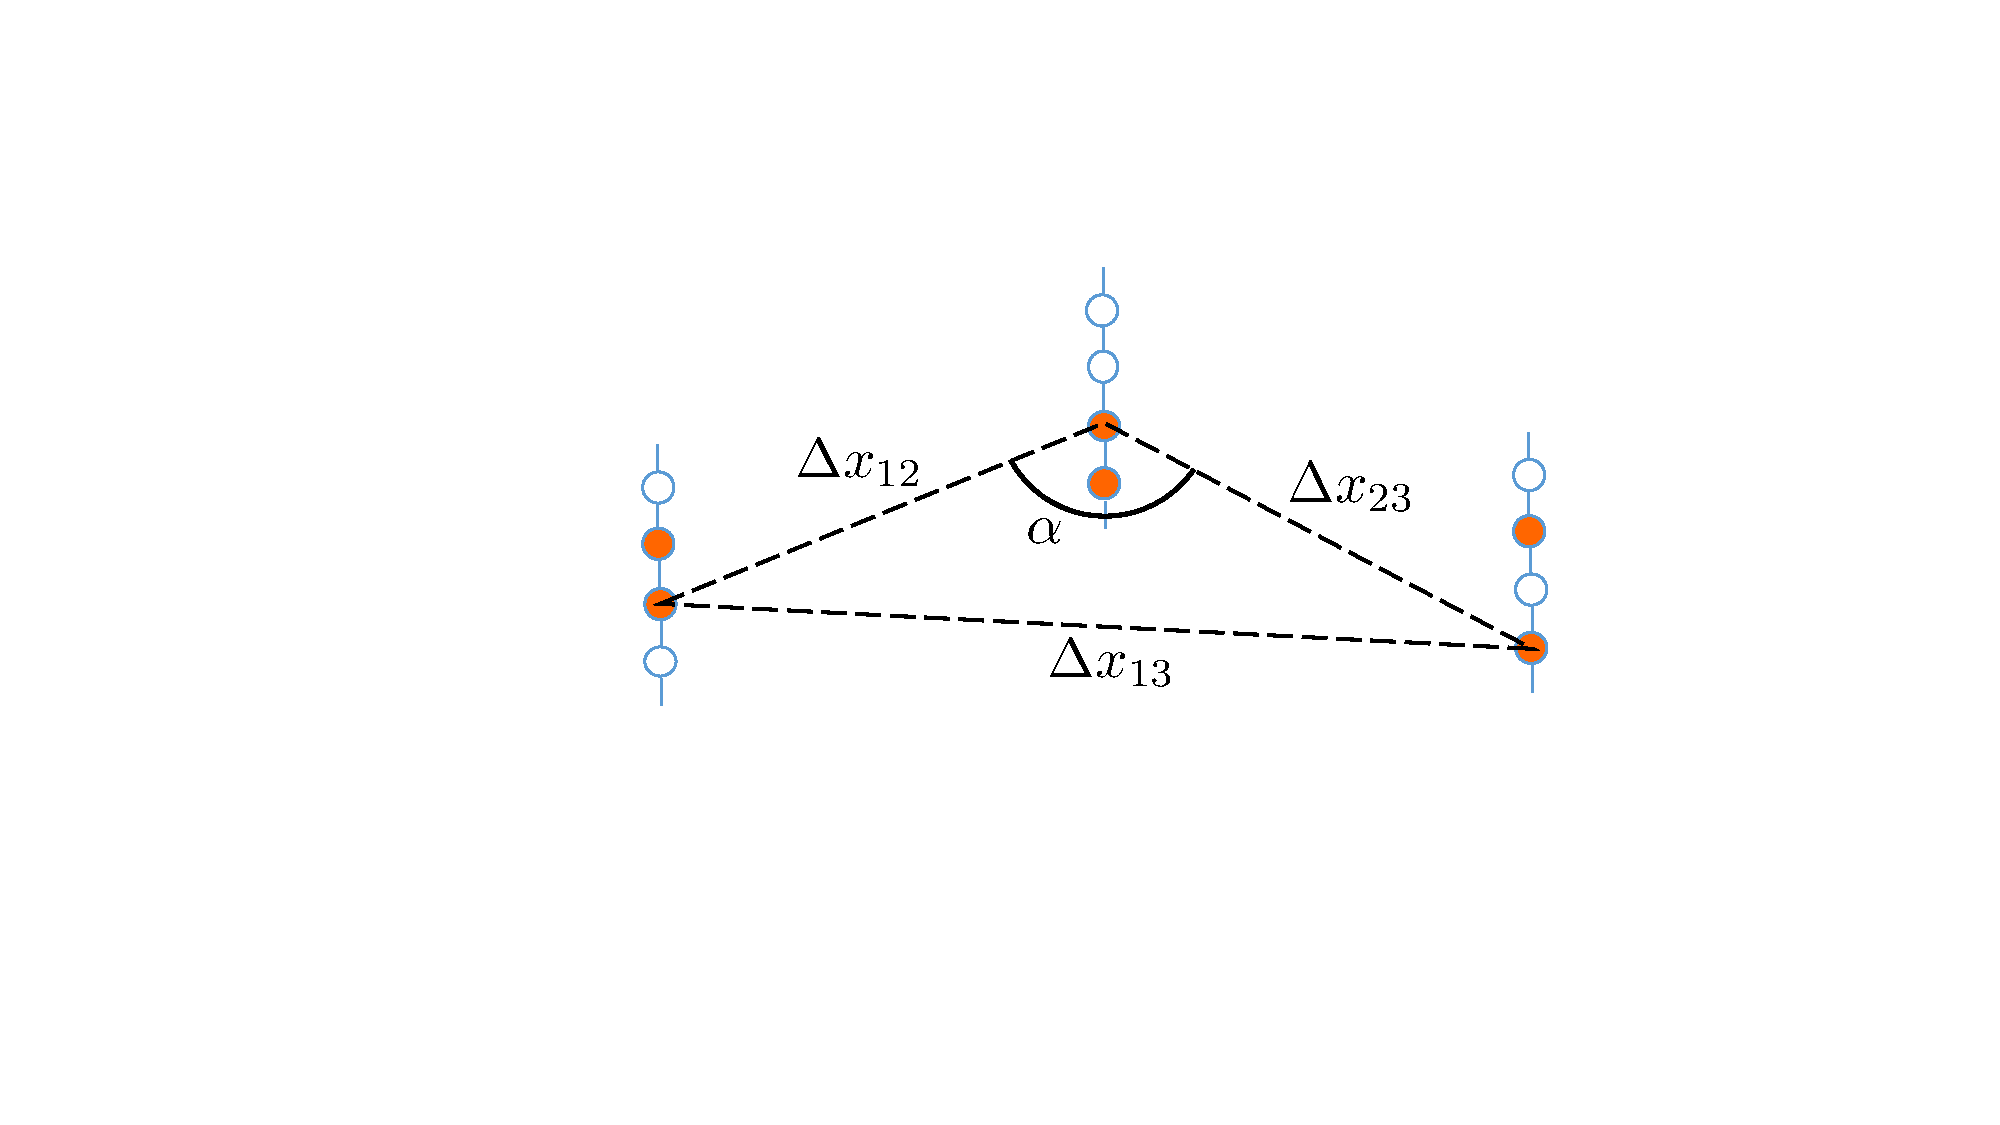
\includegraphics[width=0.6\textwidth]{graphics/online/trigger/slop.pdf}
 \caption{Geometry of a SLOP trigger triplet of HLC pairs.}
 \label{fig:slop}
\end{figure}

Other special-purpose triggers exist to collect minimum bias data of
various sorts.  The Fixed-Rate Trigger (FRT) reads out 10~ms of hit data from
the full detector at fixed intervals.  This is especially useful for studies
of DOM noise.  The Calibration Trigger selects a particular type of hit
such as special IceTop non-HLC hits that have full waveform readout, and promotes
them to a trigger. The Calibration Trigger can also be configured to
include all events due to LED flashers in cases where flasher 
operations require disabling standard triggers. Finally, a Minimum Bias
trigger can select one of every $N$ HLC hits and promote this hit to a trigger, adding
readout windows as usual; currently an IceTop Minimum Bias trigger with a
prescale factor $N$ of 10000 is active.

\begin{table}
  \centering \footnotesize
\caption{Trigger parameters (as of May 2016) and typical trigger
  rates of each algorithm.  Most rates vary seasonally with the atmospheric
  muon flux.  The merged event rate varies from 2.5 to
  2.9 kHz.}  
\begin{tabular}{lrrrrr}
  \hline Trigger & DOM set & $N$ HLC hits & Window & Topology & Rate\\
  & & & ($\mu$s) & & (Hz) \\
  \hline
  SMT & in-ice & 8 & 5 & --- & 2100\\
  SMT & DeepCore & 3 & 2.5 & --- & 250\\
  SMT & IceTop & 6 & 5 & --- & 25\\
  Volume & in-ice & 4 & 1 & cylinder (r=175m, h=75m) & 3700\\
  Volume & IceTop infill & 4 & 0.2 & cylinder (r=60m, h=10m) & 4\\
  String & in-ice & 5 & 1.5 & 7 adjacent vertical DOMs & 2200\\
  SLOP & in-ice & $N_{\mathrm{triplet}} = 5$ & $T_{\mathrm{prox}} = 2.5$, &
  $\alpha_{\mathrm{min}} = 140^\circ,\ v_{\mathrm{rel}}^{\mathrm{max}}
  = 0.5$ & 12\\
  & & & $T_{\mathrm{min}} = 0$, & &\\
  & & & $T_{\mathrm{max}} = 500$ & &\\
  FRT & all & --- & --- & --- & 0.003\\
  \hline
\end{tabular}
\label{tab:triggers}
\end{table}

Many events will satisfy more than one of the trigger conditions, sometimes
multiple times.  In order to avoid overlapping events, possibly containing
the same DOM hits, the triggers and their associated readout windows are
merged, while retaining information about the separate triggers.  The
merged trigger is referred to as the Global Trigger.

Each trigger has defined readout windows around the trigger window; all
hits from the full detector, including those DOM sets not involved in the trigger,
are requested from the StringHub components and built into events.  For the
DOM set involved in an in-ice trigger, the readout windows are appended at each end of the trigger
window, while for other DOM sets, the readout windows are centered around
the trigger start time.  Readout windows around IceTop triggers are global
and include hits from all other DOM sets before and after the trigger
window. The union of overlapping readout windows defines 
an event (Fig.~\ref{fig:trigger_readout}).  Long events such as SLOP or FRT
triggers typically contain several causally independent ``physics'' events;
these typically are re-split before reconstruction and analysis.

\begin{figure}[!ht]
 \centering
 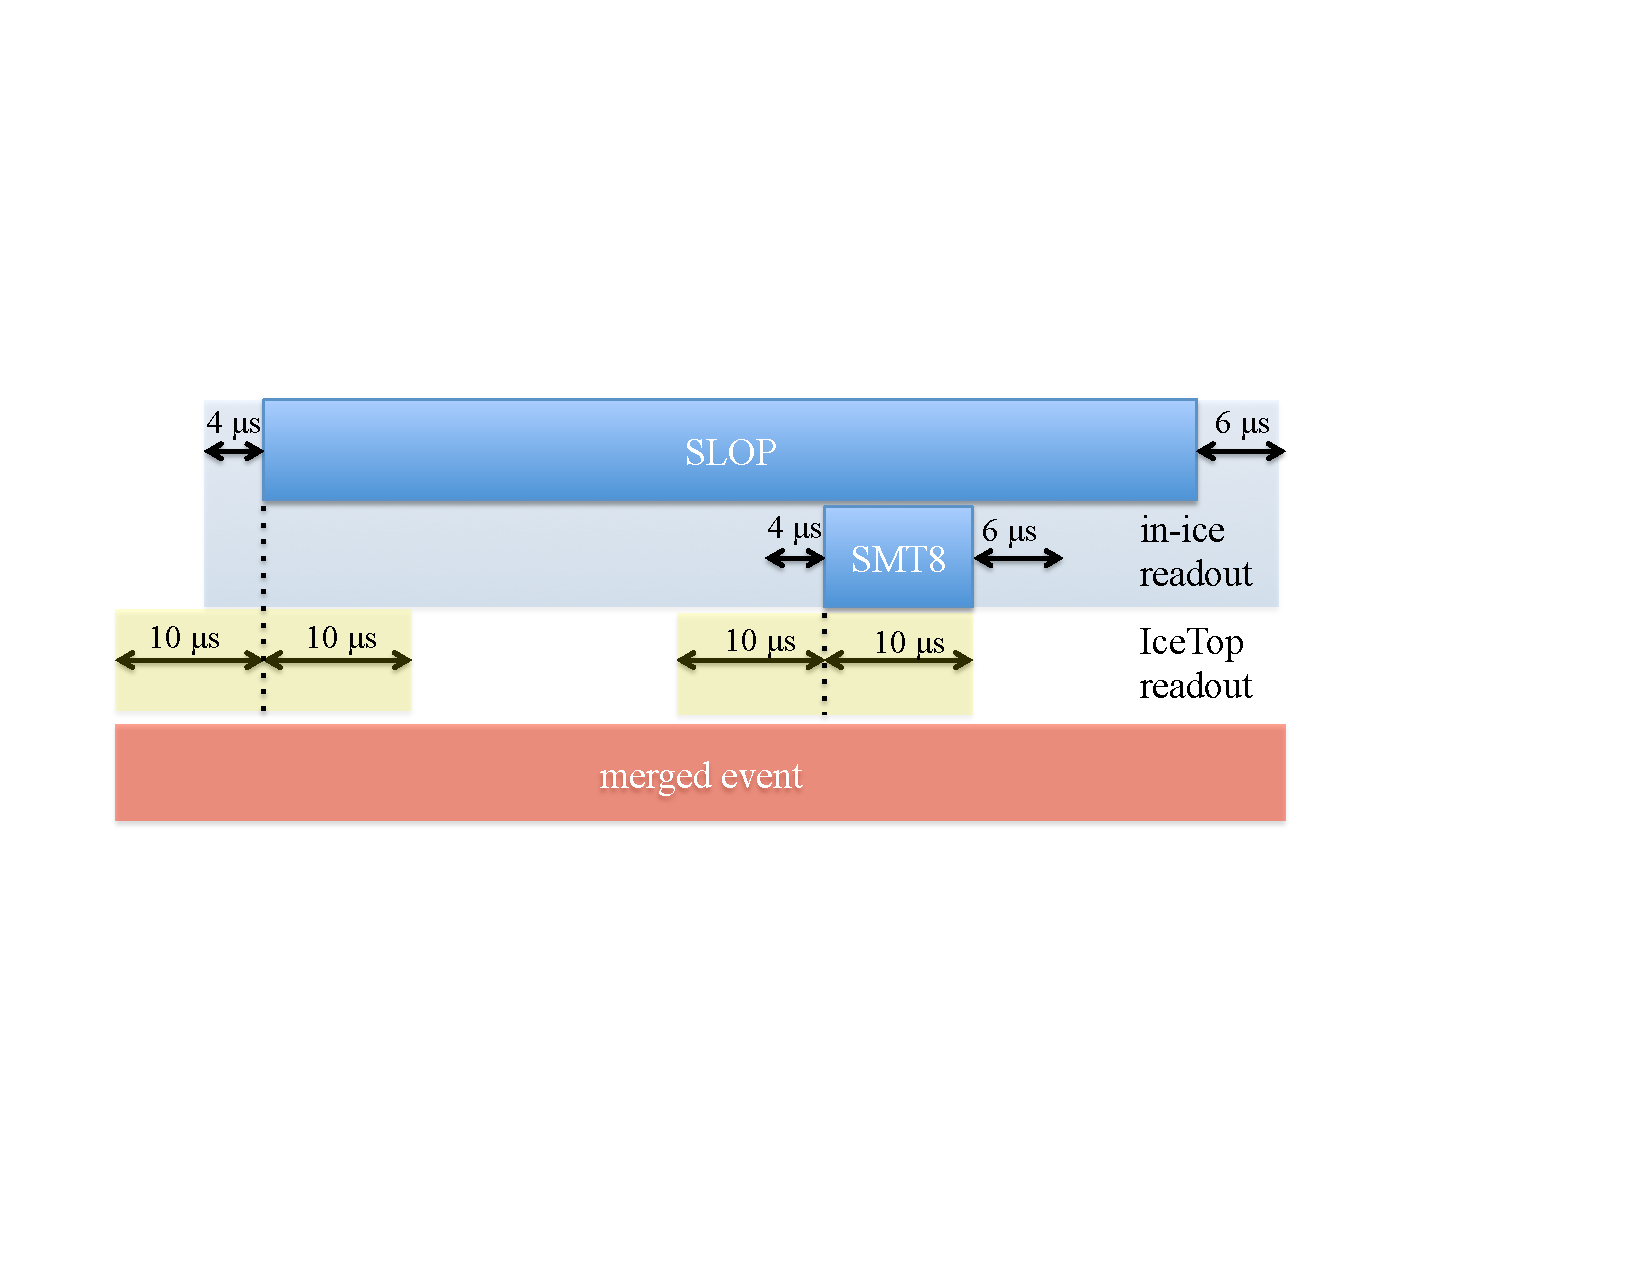
\includegraphics[width=0.8\textwidth]{graphics/online/trigger/trigger_readout}
 \caption{In-ice, IceTop, and merged readout windows for a long event
   satisfying SLOP and SMT8 triggers.}
 \label{fig:trigger_readout}
\end{figure}

% \begin{figure}[ht]
%   \centering
%   \subfloat[Sample bright event satisfying multiple triggers.  The vertical ticks
%     indicate the time of DOM hits (including SLC hits).  Trigger windows are
%     illustrated with solid horizontal lines, readout windows by dashed lines.]{
%     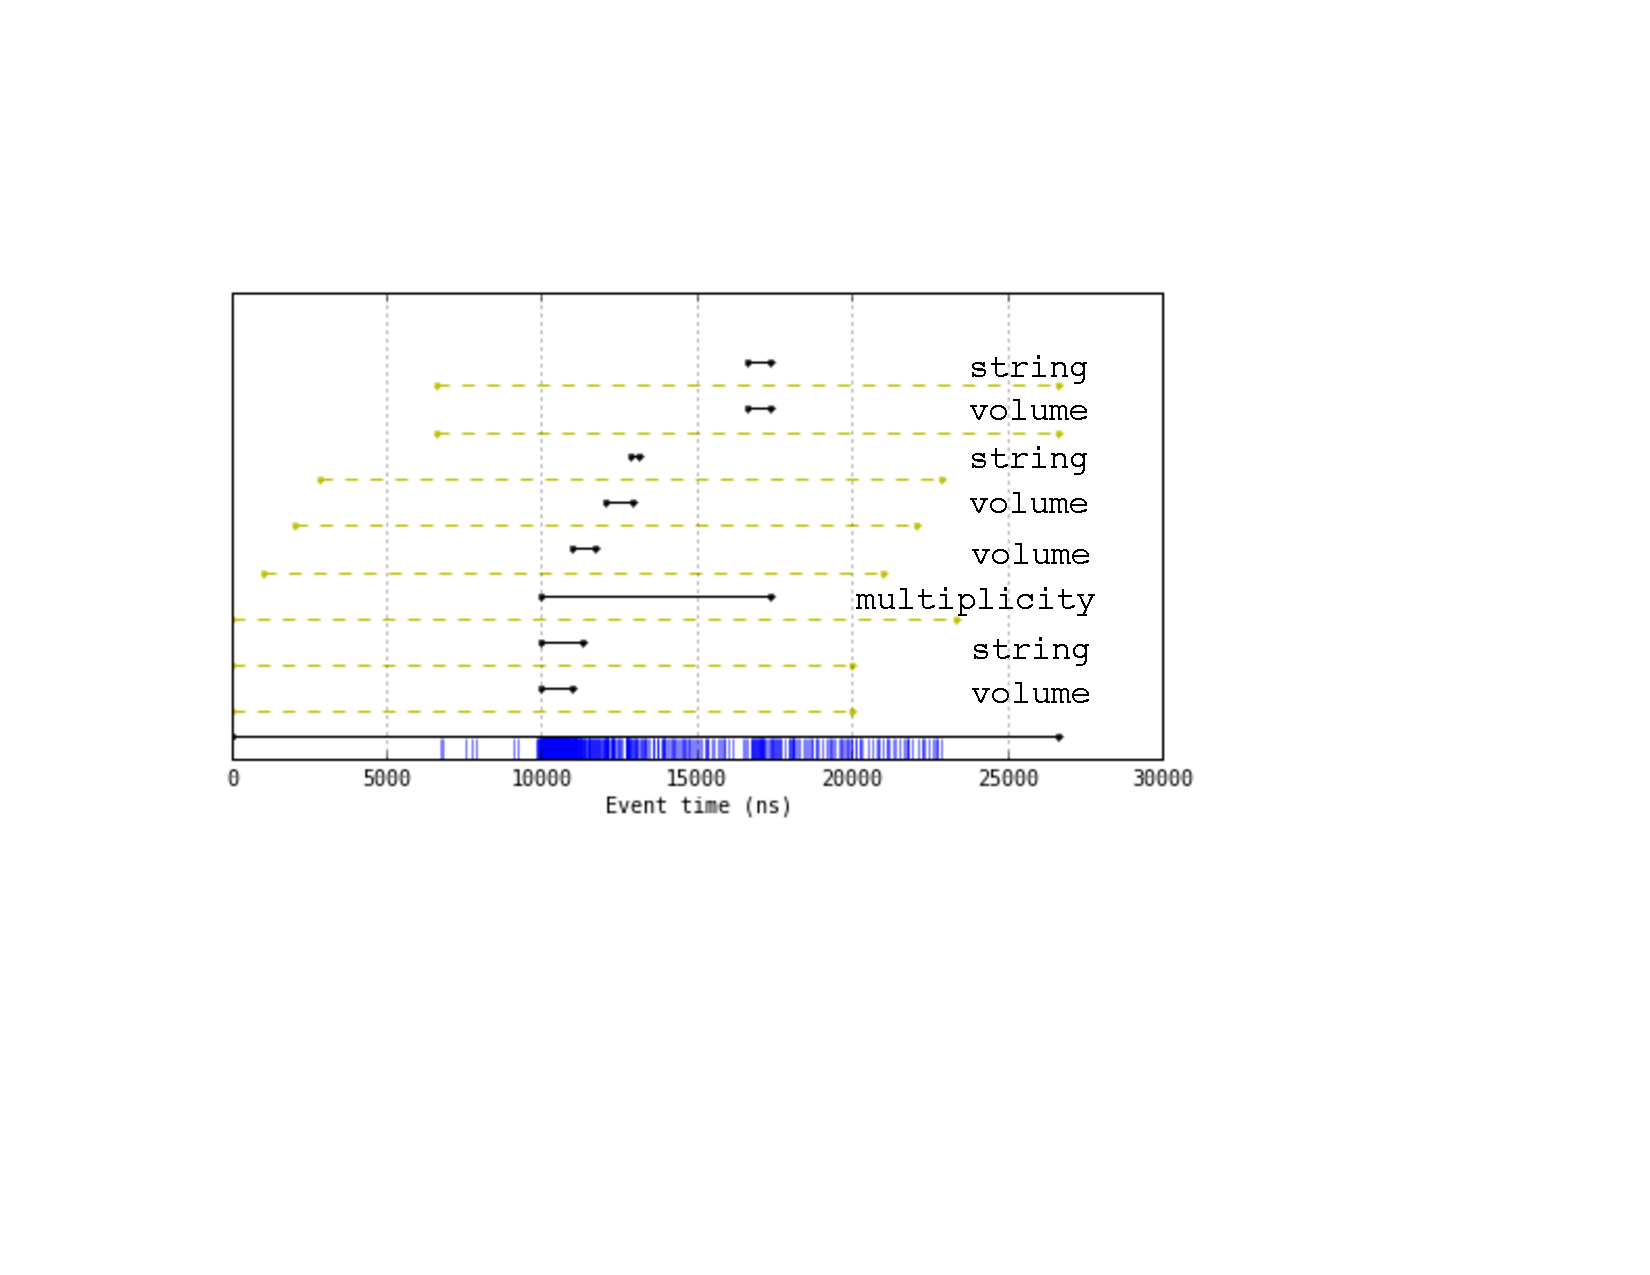
\includegraphics[scale=0.5]{graphics/online/trigger/trigger_example}
%     \label{fig:trigger_example}
%   }
%   \quad
%   \subfloat[In-ice, IceTop, and merged readout windows for a long event
%     satisfying SLOP and SMT8 triggers (not to scale).]{
%     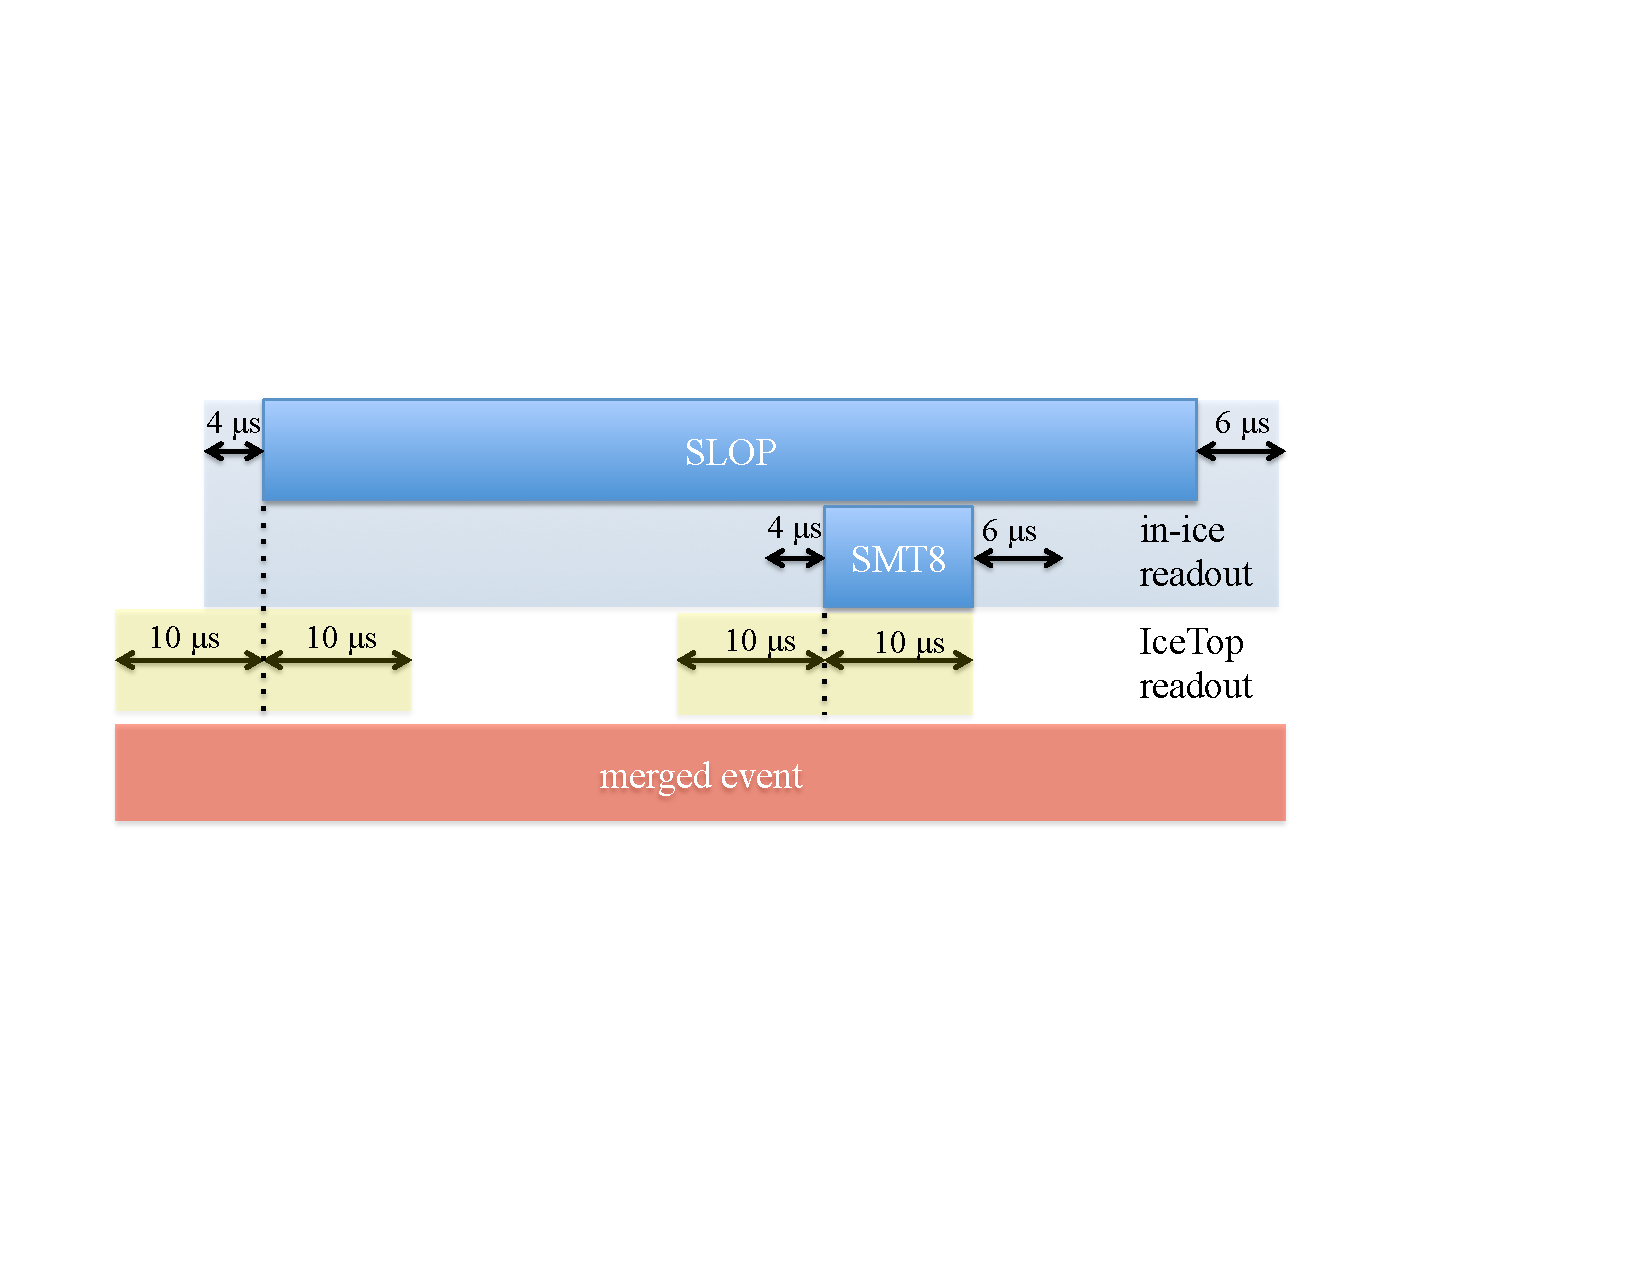
\includegraphics[scale=0.5]{graphics/online/trigger/trigger_readout}
%     \label{fig:trigger_readout}
%   }
%   \caption{IceCube trigger and readout window merging.}
% \end{figure}

\subsubsection{\label{sect:online:evbuilder}Event Builder}

The Event Builder receives requests from the Global Trigger, extracts the
individual readout windows, and sends them to the appropriate subset of the
StringHubs.  The StringHubs each send back a list of all hits within the
window. When all StringHubs have returned a list of hits, these are bundled with the trigger data into an event.

Events are written to a temporary file.  When the temporary file
reaches a preset configurable size, it is renamed to a standard unique name.  When the PnF
system sees a new file, it accepts it for processing and filtering
(Sec.~\ref{sect:online:filter}).  The total latency from detection of
photons at the DOMs to DAQ events written to disk is approximately five
seconds. 

\subsubsection{\label{sect:online:daqdomconfig}DAQ and DOM Configuration}

The configuration of the DAQ is managed by two sets of XML files: a cluster
configuration file and a hierarchical tree of run configuration files.

The cluster configuration file contains system-level settings used to
launch the DAQ, such as component host servers, startup paths, command-line
options, etc.  Components (other than StringHub) can easily be moved to
different hosts for troubleshooting, load balancing, and maintenance.

Run configuration files list the trigger and DOM configuration files to be
used for taking data.  The trigger configuration file specifies
configuration parameters for all 
trigger components (in-ice, IceTop, and global) used in a run.  These
include the list of algorithms run by each trigger component, along with
readout window sizes and any other configurable parameters (multiplicity
threshold, trigger period, prescale factor, etc.).

DOM configuration files (one per hub) list all DOMs that contribute to
the data-taking run.  All configuration parameters for each DOM are
specified, including PMT high voltages, ATWD operating parameters,
discriminator thresholds, local coincidence settings, baselines and others.

Run configuration files (including trigger and DOM files) are versioned and
frozen once used for data-taking.  All relevant configuration parameters
are also stored in a database for use in analysis.

An additional geometry XML file contains the $(x,y,z)$ and (string,
position) coordinates of the DOMs, needed by the Trigger components.  DOMs
are individually identified by the DAQ using an ID generated from a
component device identifier on the DOM Main Board.  This ensures that cabling changes
on a DOMHub do not result in changes in data-taking or errors in the geometry.

\subsubsection{Component Control}

The DAQ components are managed by a single ``command-and-control'' daemon,
CnCServer, that manages and monitors components and acts as the main
external interface to the DAQ.  It uses a standard component interface to query and
control the components, and a separate interface for components to expose
internal data used for monitoring the health of the detector or for
debugging purposes.

CnCServer dynamically discovers the detector components during a launch
phase, and instructs them to connect to each other as needed.  Using the
run configuration files, it then distributes each component configuration
appropriately.  The components are then started to begin a data-taking run.
When a run is in progress, CnCServer regularly checks that components are
still active and that data are flowing between components.

%CnCServer starts out knowing nothing about the detector components.  During the
%DAQ's launch phase, components are given the host and port used by CnCServer.
%When components start up, each one sends CnCServer its name, host/port pairs,
%and the types of inputs and outputs it expects, and CnCServer adds them to its
%internal list.

%To start a run, CnCServer is given the name of the run configuration.  That
%run configuration may include all components or only a subset.  Using
%that file, CnCServer builds a list of components required for the run.
%Each of the included components is told to connect to their downstream
%neighbor, then to use the run configuration to initialize as appropriate
%(configure DOM hardware, initialize trigger algorithms, etc.).
%Once all components are successfully
%configured CnCServer instructs them to start, working its way from the Event
%Builder back to the String Hubs.

%When a run is in progress, CnCServer regularly checks that components are still
%active and that data are flowing between components.  If it detects a problem,
%it stops the run and relaunches all the components.  CnCServer also
%periodically collects all components' monitoring data and writes it to
%monitoring files which can be used for post-mortem diagnosis of detector
%failures.

\subsubsection{\label{sect:SNDAQ}Supernova Data Acquisition System}

The IceCube DAQ has a parallel triggering and analysis pathway designed
specifically for the detection of the many $O(10)$ MeV neutrinos from a
Galactic core-collapse supernova.  In the case of such an event, these
neutrinos will produce interactions in
the detector that, individually, are too dim to trigger the standard DAQ,
but because of their high number, can cause a coherent rise in the
individual hit rates of the DOMs~\cite{IC3:supernova}.

Each DOM monitors its hit rate and sends a stream of binned counts, using a
bin width of 1.6384~ms ($2^{16}$ clock cycles at 40 MHz).  An artificial
deadtime of $250\ {\mu}\mathrm{s}$ is applied after each hit to reduce the
impact of correlated hits (Sec.~\ref{sect:darknoise}).  Each
StringHub collects the rate stream of each DOM, supplies UTC-based timestamps,
and forwards the streams to the Secondary Builder.

The supernova DAQ (SNDAQ) system receives the Secondary Builder stream,
rebins the individual DOM rates, and monitors the sum of rates over several
timescales for a significant rise.  This analysis is described in
detail in Ref.~\cite{IC3:supernova}.  One complication is that light
deposition from cosmic-ray muons distorts the significance
calculation.  To correct for this, the trigger rate of the standard DAQ is
continuously sent to SNDAQ, and any significant alert is corrected
\cite{IC3:icrc15_sndaq}.  At a high significance threshold, the capture of
all untriggered data around the alert time is initiated using the HitSpool
system (Sec.~\ref{sect:hitspool}), and the Supernova Neutrino Early Warning
System (SNEWS) \cite{SNEWS} is notified.  SNDAQ latency of approximately 7
minutes is dominated by the sliding window algorithm used to determine
average DOM rates. 

\subsubsection{\label{sect:hitspool}HitSpool Request System}

In the event of a significant transient event, subsystems such as SNDAQ can
request all untriggered DOM hits from the detector in 
a particular time interval by sending requests to a HitSpool Request daemon. Presently,
the HitSpool Request System has three clients; 
their basic characteristics are described in
Table~\ref{tab:hsclients}.  The central daemon passes the request on to 
every DOMHub, where hits in the requested time
interval are gathered and forwarded to a ``sender'' component.  The hits
are then bundled and transferred to the Northern Hemisphere for further analysis.

The time windows of SNDAQ HitSpool data requests are based on the
statistical significance of the alert and are shown in
Table~\ref{tab:hsclients}. The online High Energy Starting Event (HESE) 
analysis system requests HitSpool data from a symmetrical time window of
1~s around events with a total deposited charge of greater than 1500~PE.
The recently implemented HitSpool client for solar flare analyses is
triggered externally by significant Fermi Large Area Telescope (LAT) events~\cite{fermilat:flare}
and requests HitSpool 
data from a symmetrical time window of one hour around the trigger
time. Unlike the other two clients, these data sets are not transferred
over the satellite due to their size but are stored locally on disk, with
transmission over satellite only pursued in extraordinary cases.

\begin{table}
  \caption{HitSpool data-requesting services and request characteristics.
    The SNDAQ quantity $\xi$ is related to the statistical significance of
    the rate fluctuation.}
  \centering
  \footnotesize
\begin{tabularx}{\textwidth}{lcXXXX}
  \toprule Client & Trigger Threshold & Time\newline Window & Request
  Length & Raw \newline Data Size & Frequency \\
  \midrule
  SNDAQ & $7.65 \le \xi < 10$  & $[-30\,\mathrm{s},+60\,\mathrm{s}]$ &
  $90 \,\mathrm{s}$& $15 \,\mathrm{GB}$&
  $0.5/\mathrm{week}$ \\
   & $\xi \ge 10$ &  $[\pm250\,\mathrm{s}]$ & $500\,\mathrm{s}$ & $85
  \,\mathrm{GB}$ & $0.0006 / \mathrm{week}$ \\
  HESE & $1500 \,\mathrm{PE} $ &
  $[\pm0.5\,\mathrm{s}]$& $1\,\mathrm{s}$ & $175\,\mathrm{MB}$ &
  $4/\mathrm{day}$ \\
   & 6000 PE & & & & $1/\,\mathrm{month}$ \\ 
  Solar Flare & Fermi-LAT & $[\pm30\,\mathrm{min}]$ & $1\,\mathrm{h}$&
  $~600\,\mathrm{GB}$& $ 7 / \mathrm{year}$ \\
  & significant event & & & & 
  \\ \bottomrule
\end{tabularx}
\label{tab:hsclients}
\end{table}

\subsection{\label{sect:online:filter}Online Processing and Filtering}

\subsubsection{Overview}

The online Processing and Filtering (PnF) system handles
all triggered events collected by the DAQ
and reduces the data volume to a level that can be accommodated in our
satellite bandwidth allocation (about 100 GB/day).  This treatment
includes application of calibration constants, event
characterization and selection, extraction of data quality monitoring
information, generation of realtime alerts for events of astrophysical
interest, and creation of data files and metadata information for long-term
archiving.  The PnF system is a custom software
suite that utilizes about 20 standard, multi-processor servers located in
the SPS computing cluster.  

The first step in the analysis of triggered events is the calibration of
the digitized DOM waveforms, as described in Sec.~\ref{sec:waveformcal}.
The geometry, calibration, and detector status (GCD) information needed to
process the data is stored in a database.  Next, each DOM's waveform is
deconvolved using the known DOM response to single photons to 
extract the light arrival time and amplitude information~\cite{IC3:ereco}.
This series of time and amplitude light arrival information for each DOM is
the basis for event reconstruction and characterization.  PnF encodes this
information in a compact data format known as the Super Data
Storage and Transfer format (SuperDST); this format uses only 9\% of the storage
size of the full waveform information.  The encoding does introduce a
small level of discretization error to the data, measured to be 1.1~ns in time and
0.04~PE in charge, smaller than the calibration uncertainties on these
values.  Any DOM readout whose SuperDST information is found not to be a
good representation of the original waveform, or sees large amounts of
light, also has the full waveform data saved in addition to the
SuperDST record.

% JVS internal study on discretization:  
% https://events.icecube.wisc.edu/getFile.py/access?contribId=140&sessionId=4&resId=0&materialId=slides&confId=33

Each event is then characterized with a series of reconstruction
algorithms that attempt to match the observed patterns of recorded light in
the SuperDST with known patterns of light from track and shower event
hypotheses~\cite{IC3:ereco}.  The reconstructed vertex position, direction,
energy, and the goodness-of-fit are used to select interesting events by various
filter selections.  The filter criteria are set by the collaboration
each year and are tuned to select events of interest to specific
analyses.  Each year there are about 25 filter selections in
operation; as of 2016, approximately 15\% of all triggered events are
selected by one or more filters.  Some of these filters are designed to search for
neutrino events of wide astrophysical interest to the scientific community
and trigger alerts that are distributed to followup observatories
worldwide~\cite{Abbasi:2011ja,Aartsen:2015trq}.

The PnF system also extracts and aggregates data quality and monitoring
information from the data during processing.  This information includes
stability and quality information from the DOM waveform and calibration
process, rates of DOM readouts, and rates and 
stability information for all detector triggers and filters.  This
information is aggregated for each data segment and reported to the IceCube
Live monitoring system (Sec.~\ref{sec:online:icecubelive}).

Finally, the PnF system generates several types of files for satellite
transmission and for long term archival. These
include:   
\begin{enumerate}
\item Filtered data files containing events selected by the online filter
  selections.  These events generally only include the SuperDST version of
  the DOM information and results from the online event reconstructions.
  The files are queued for satellite transmission to the IceCube data
  warehouse in the Northern Hemisphere by the data handling system.
\item SuperDST data files containing the SuperDST version of DOM readout
  information for all triggered events as well as summary information from
  the online filtering process.  This file set is intended as the long-term
  archive version of IceCube data.
\item Raw data files containing all uncalibrated waveforms from all DOMs for
  every event.  %This large data set is saved until final data quality
%  assurance on the SuperDST sample can be completed.
\end{enumerate}

During normal operations, the DAQ produces a raw data output of
$\sim$1 TB per day, resulting in a raw data file 
archive of the same size.  The SuperDST and filtered data archive, after
data compression, are $\sim$170 GB/day and $\sim$90 GB/day, respectively.

\subsubsection{System Design}

The PnF system uses a modular design based on
a central master server node and a scalable number of data processing client
nodes.  The central master server handles data distribution and
aggregation tasks (requesting data blocks from the DAQ, collating event
SuperDST, reconstruction, filter, and monitoring information and writing
data files), while the clients handle the per-event processing
tasks (event calibration, reconstruction, analysis, and filtering).

The system is built upon the IceCube analysis software framework,
IceTray~\cite{DeYoung:2005zz}, allowing standard IceCube algorithms to be
used online without modifications.
Additionally, the system uses the Common Object Request Broker Architecture
(CORBA) system as a means for controlling, supervising and interconnecting
the modular portions of the system.  Specialized CORBA classes allow
data to stream from one component to another using IceTray formats.
Clients can also be easily added and removed as needed to meet the
processing load.

\subsubsection{Components}

The flow of triggered event data in the PnF
system is shown in Fig.~\ref{fig:online_pnf_internals}.  Standard
components include: 
\begin{enumerate}
\item DAQ Dispatch, a process to pick up event data from the DAQ data cache
  and forward to the Central Server components. 
\item Central Servers, which
  receive data from the 
  DAQ Dispatch event source, distribute events to and record results
  returning from the PnF client farm, and send events to Writer components.
  Typically there are four servers used in operation.
\item Filter Clients, where the core calibration, reconstruction and
  filtering processes are applied to each triggered event.  Up to 500 of
  these clients operate in parallel to filter 
  events in real time.
\item GCD Dispatch, a database caching system to prevent the
  Filter Client processes from overwhelming the GCD database at run transitions.
\item File Writers, responsible for creation of files and metadata for
  the data archive.  There is one writer component for each file type created.
\item Online Writer, responsible for extracting event reconstruction and
  filter information from the data for events of astrophysical interest and
  sending this information out in real time via the IceCube Live alert
  system.
\item Monitoring Writer, responsible for aggregating per-event monitoring
  information, creating histograms, and forwarding to the IceCube Live
  monitoring system.
\item Filtered Data Dispatch and FollowUp Clients, responsible for
  looking for bursts of neutrino events on timescales from 100 seconds up
  to 3 weeks in duration.  Any significant burst of neutrinos found generates alerts
  sent to partner observatories worldwide.
\end{enumerate}

\begin{figure}[!ht]
 \centering
 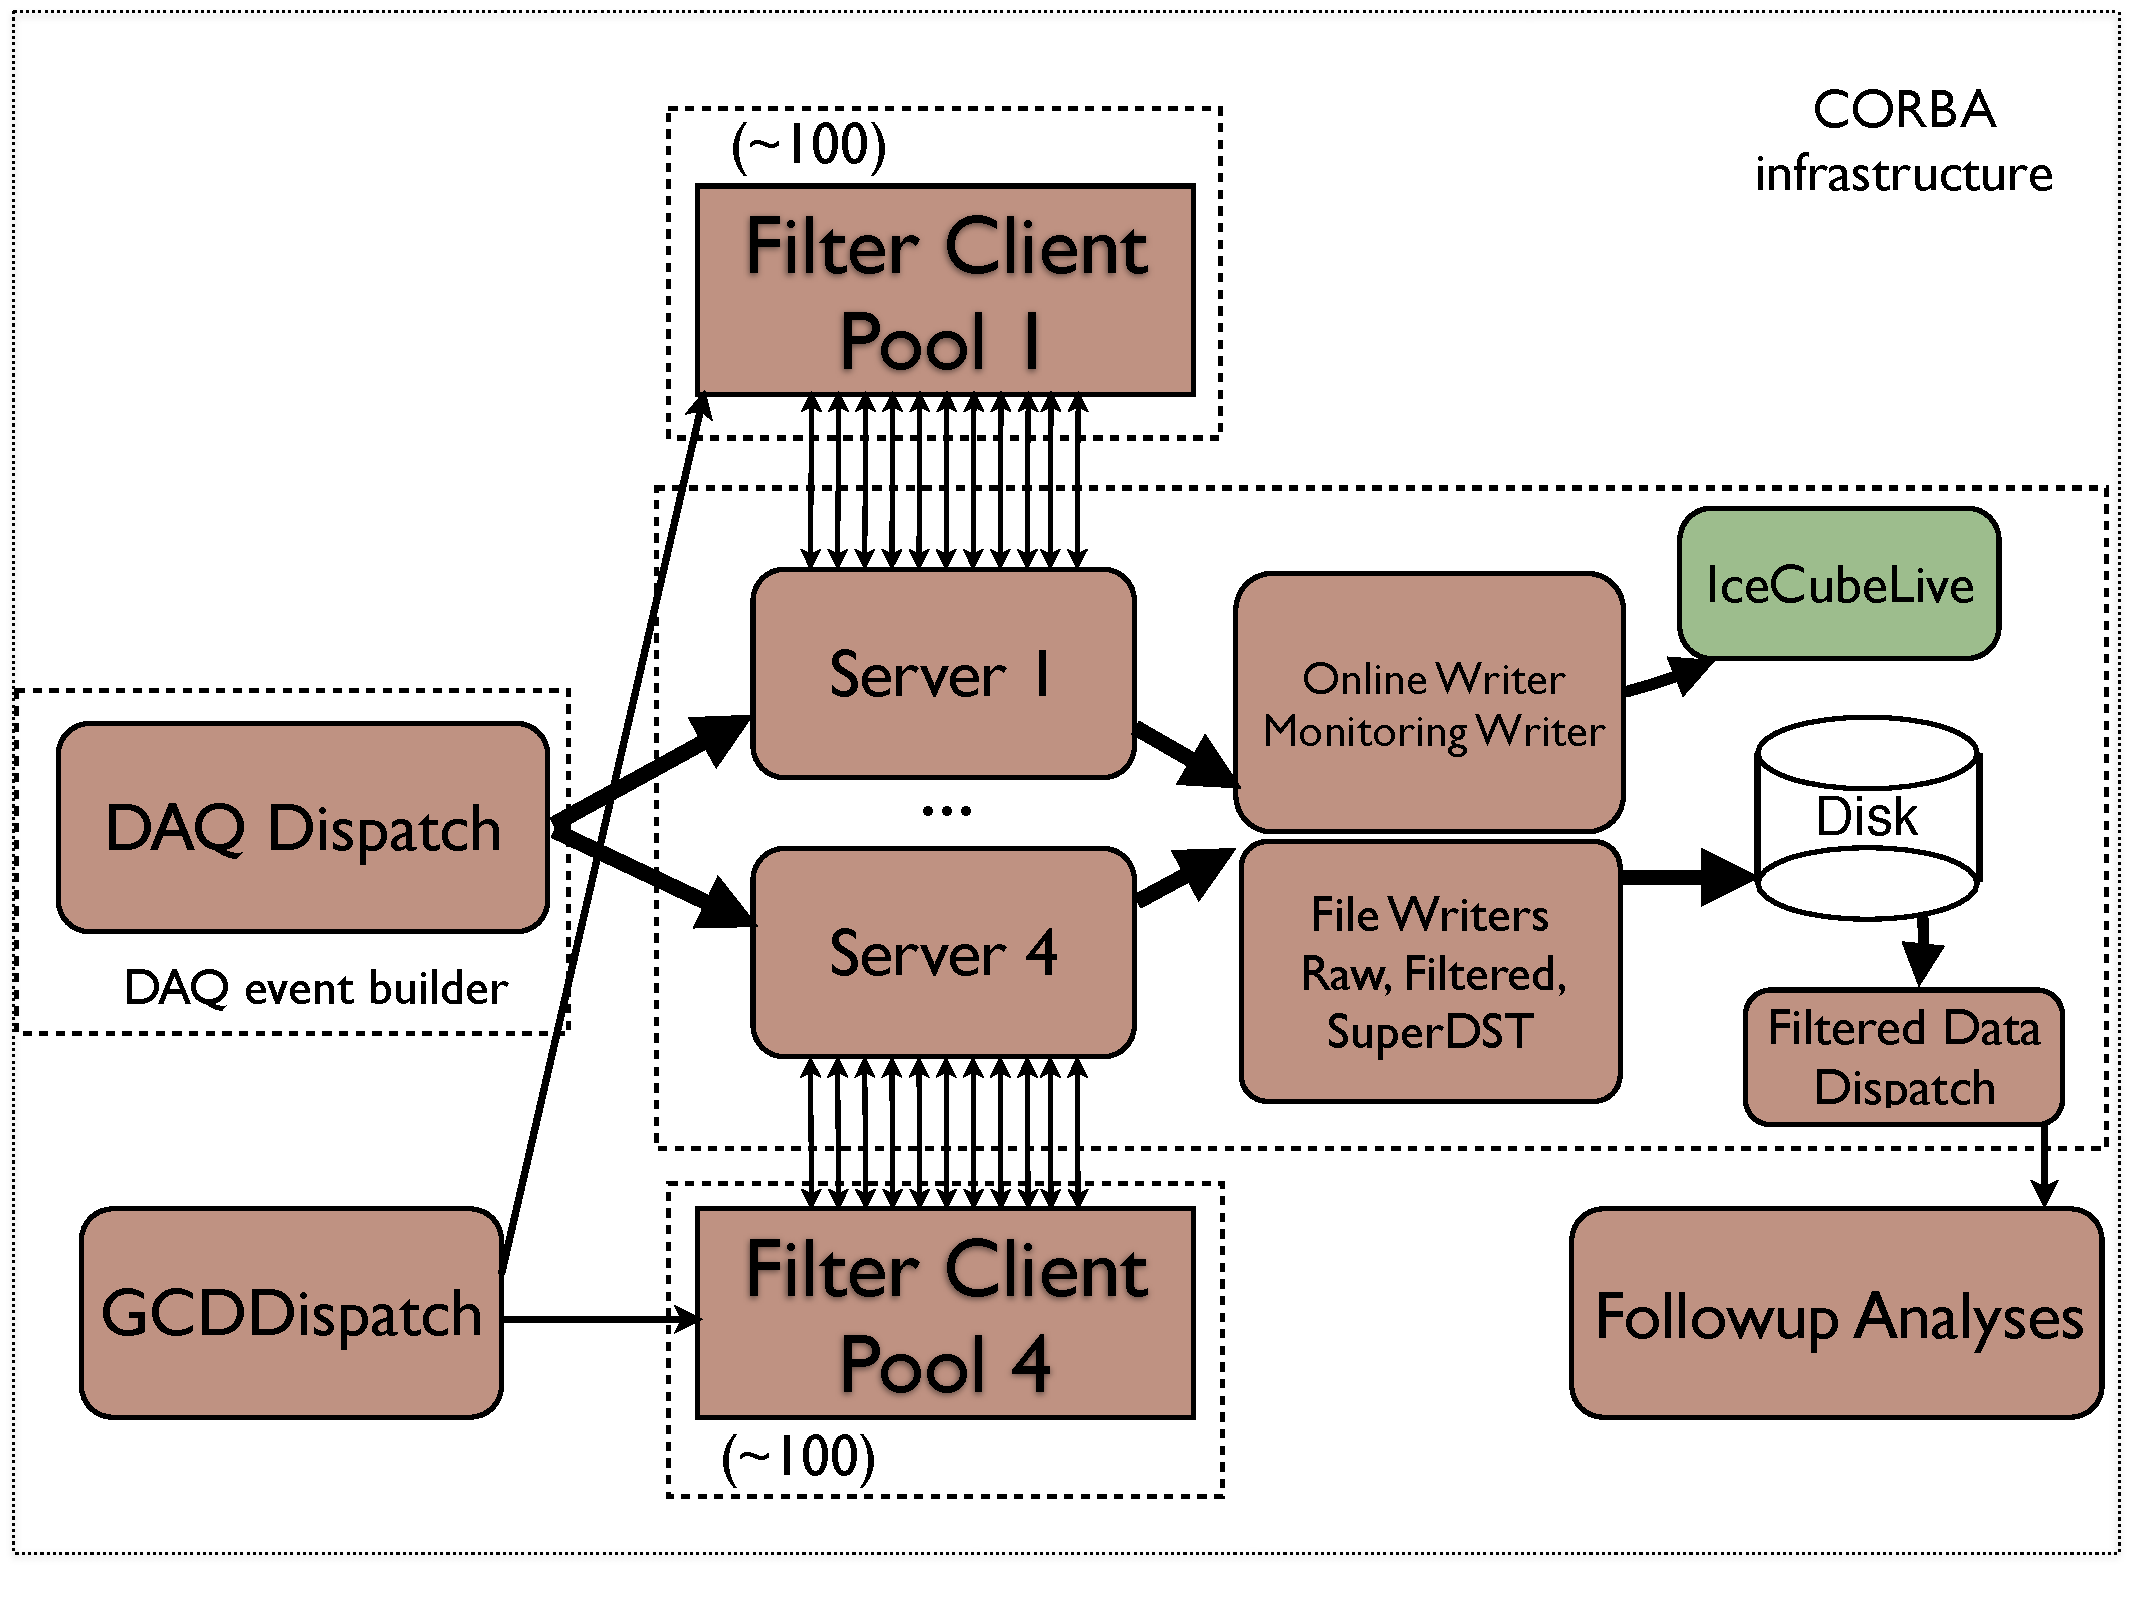
\includegraphics[width=0.8\textwidth]{graphics/online/pnf/PnF_Internals.pdf}
 \caption{Internal components of the PnF
   system.  Arrows show the flow of data within the system.}
 \label{fig:online_pnf_internals}
\end{figure}

\subsubsection{Performance}

The PnF system is designed to filter triggered events as quickly as
possible after collection by the data acquisition 
system.  A key performance metric is processing system latency, defined as the duration
of time between the DAQ trigger and the completion of event
processing and filtering.  A representative latency history for the system is
shown in Fig.~\ref{fig:online_pnf_latency}, showing typical system
latencies of about 20 seconds.

\begin{figure}[!ht]
 \centering
 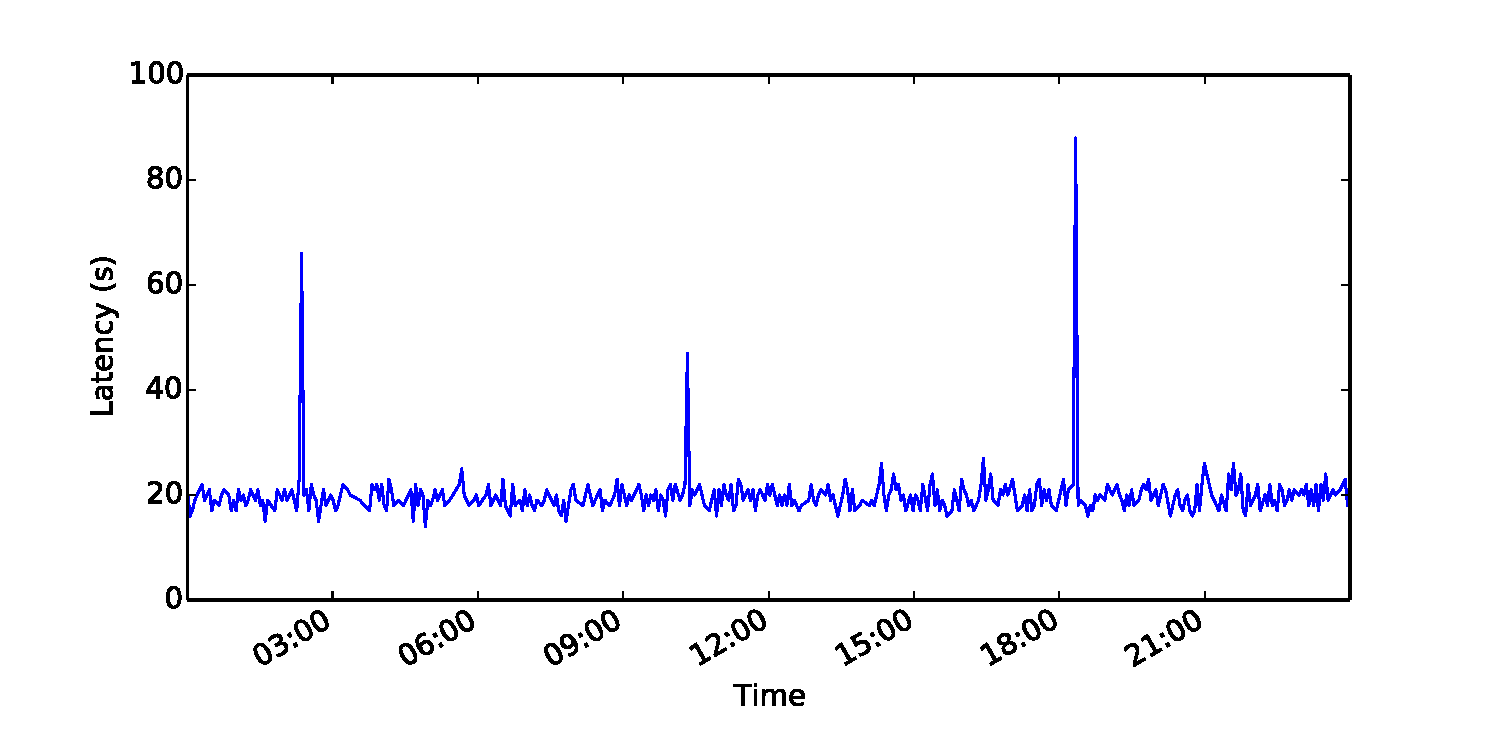
\includegraphics[width=0.85\textwidth]{graphics/online/pnf/pnf_latency_160627.pdf}
 \caption{Typical PnF system latency for a
   24-hour period.  The latency is defined as the time between DAQ trigger
   time and time when the online filtering processing is complete.  The
   spikes in latency correspond to DAQ run transitions, when
   geometry, calibration, and detector status information is updated and
   distributed to the filtering clients.}
 \label{fig:online_pnf_latency}
\end{figure}

The filter selections used have been relatively stable over several years
of operation of the completed IceCube detector, with most seeing only minor
updates at the 
start of each season.  The majority of physics analyses derive from a small
set of core filters, including:

\begin{enumerate}
\item A muon track filter that searches for high-quality track events from all
  directions.  Up-going events for all triggered energies are selected,
  while only high-energy 
  down-going tracks are selected to avoid the large background of
  down-going atmospheric muons at lower energies.  These selected events
  are frequently used as the input to point source and transient neutrino searches.
\item A shower event filter that searches for events producing large energy
  depositions in or near the instrumented volume.  These selected events are
  frequently used as the input to searches for high-energy shower events arising from
  atmospheric and astrophysical neutrinos.
\item A high-charge filter that searches for any event depositing a
  large amount of energy leading to a recorded charge of $\geq1000$
  photoelectrons in the 
  instrumented volume.  While having a large overlap with the muon track
  and shower filters at high energies, this filter targets the highest
  energy neutrino events of all types. The selected events are used as
  inputs to searches for high-energy astrophysical and cosmogenic
  neutrinos as well as for relativistic magnetic monopoles.
\item Cosmic ray filters that search for extended air-shower events in
  IceTop.  The selected events are used as inputs to analyses 
  targeting the flux, spectrum, and composition of the primary cosmic rays
  observed in the Earth's atmosphere.
\item A DeepCore contained event filter that searches for contained, lower-energy
  neutrino events (in the range of 10--100 GeV) from atmospheric neutrino interactions
  that are contained within the more densely instrumented DeepCore region.
  The selected events are used as inputs to analyses that measure
  neutrino oscillation effects and search for indirect signatures of dark matter.
\end{enumerate}

\noindent Other filters are employed for more specialized searches, as well as for minimum bias selections.

\subsection{\label{sect:online_jade}Data Handling}

The bulk of South Pole Station data traffic is handled by geosynchronous
satellite links.  Due to the location, only
geosynchronous satellites with steeply inclined orbits reach far enough
above the horizon to establish a link.  For a given satellite, this link
provides four to six hours of communications once per sidereal day.
Multiple satellites are currently utilized by the
U.S.~Antarctic Program, providing a window of about 12 hours of connectivity with
bandwidth of 250 Mbps for uni-directional data transfer and bandwidth
of 5 Mbps for bi-directional internet connectivity.  For the remainder of the day, Iridium
communication satellites allow limited voice and data connectivity and provide up to 2.4
kbps of bandwidth per modem.

IceCube incorporates Iridium modems into two separate systems, the legacy IceCube
Teleport System (ITS) and the IceCube Messaging System (I3MS).  ITS uses
the Iridium Short Burst Data mode to send short 
messages of 1.8 kB or smaller with a typical latency (transmission time) of 30 seconds.
Messages may either originate or terminate at the ITS Iridium modem at the
South Pole.  Messages also contain a recipient ID indicating the intended
host to receive the message, allowing a many-to-many communications
infrastructure between systems running at the South Pole and systems in the
Northern Hemisphere.  ITS was retired in 2016.

The newer IceCube Messaging System (I3MS), deployed in 2015, incorporates
multiple Iridium modems and uses the Iridium RUDICS data mode, providing a
2.4 kbit/s bidirectional serial stream per modem and a minimum latency of
about 1.5 seconds.  I3MS runs as a daemon on both ends of the link, accepts
messages via the ZeroMQ distributed messaging protocol, and transports
those messages across the link based on message priority and fair sharing
of bandwidth among all users. I3MS message recipients listen for messages
using ZeroMQ publish-subscribe (PUB-SUB), allowing a given message to be
sent to multiple recipients.  I3MS also provides low-bandwidth secure shell
(ssh) connectivity to the South Pole, allowing off-site operators
access to SPS in the case of detector issues.

Data handling is provided by three servers running the Java Archival and
Data Exchange (JADE) software. JADE is a
recent Java-based reimplementation and expansion of earlier software, the
South Pole Archival and Data Exchange (SPADE).  JADE has 
four primary tasks: data pickup, archiving, satellite transmission, and
real-time transmission. The three servers operate independently of one
another, and each is capable of separately handling the nominal
data volume; thus, data handling can continue seamlessly in case of
hardware failure or maintenance. 

JADE is configured with a number of input data streams, 
each consisting of a data server, a dropbox directory, and a filename pattern.  The
data stream dropbox directories are checked on a regular basis for new
files.  File completion is indicated by the producer creating a matching
semaphore file.  For each file, a
checksum calculated on the data server is compared to a checksum calculated
on the JADE server.  After validation, the original data file is removed
from the pickup location. 

Files are then routed according to the configuration of their
data stream, either transmitted via satellite link or 
archived locally.  Archival data
were formerly written to Linear Tape Open (LTO) tapes; the tape system was
retired in 2015, and archival data are now written to disks.
All of the archival data are buffered on the server until the storage medium
is full. In case of media failure, the buffered files can be 
immediately written to new archival media with a single command.

Data streams intended for satellite transfer are queued separately.  
JADE combines multiple smaller files or splits large files to create $\sim1$
GB bundles, allowing satellite link operators to manage the daily data
transmission.  A configurable number of bundles is then transferred to the
satellite relay server.  If satellite transmission is temporarily
interrupted, the excess bundles are staged on the JADE server. 

Small files ($<$50 KB) with high priority are sent via
the I3MS Iridium link.  In cases where the real-time link is not available, I3MS
will queue the messages to be sent when the link becomes available. All
I3MS messages are also sent to JADE to send via the geosynchronous satellite link to
ensure delivery if the Iridium link should be unavailable for an extended
period of time.

\subsection{\label{sec:online:icecubelive}IceCube Live and Remote Monitoring}

IceCube operations are controlled and monitored centrally by IceCube Live.
IceCube Live consists of two major components: LiveControl,
responsible for controlling data-taking operations and collecting
monitoring data, and the IceCube Live website, responsible for processing
and storing monitoring data as well as presenting this data in webpages and
plots that characterize the state of the detector.

\subsubsection{LiveControl}

LiveControl is responsible for controlling the state of DAQ and PnF, starting and
stopping data-taking runs, and recording the parameters of these runs.
Human operators typically control the detector and check basic 
detector status using a command-line interface to the LiveControl
daemon. Standard operation is to 
request a run start, supplying a DAQ run configuration 
file.  LiveControl then records the run number, configuration, start time,
etc. and sends a request 
for DAQ to begin data-taking.  After data-taking commences successfully,
LiveControl waits a specified amount of time, generally eight hours, then
stops the current run and automatically starts a new run using the same
configuration.

This cycle continues until stopped by a user request or a
run fails.  In case of failure, LiveControl attempts to restart data-taking
by starting a new run.  Occasionally a hardware failure occurs, and a new
run cannot be started with the supplied configuration because requested
DOMs are unpowered or temporarily unable to communicate.  In this case,
LiveControl cycles through predefined partial-detector 
configurations in an attempt to exclude problematic DOMs.  This results in
taking data with fewer than the full number of available strings, but it
greatly reduces the chance of a prolonged complete outage where no IceCube
data are recorded.

A secondary function of LiveControl is the collection, processing, and
forwarding of monitoring data from DAQ, PnF, and other
components.  The associated JavaScript Object Notation (JSON) data are
forwarded to LiveControl using the ZeroMQ protocol and queued internally 
for processing.  Certain monitoring quantities indicate serious problems with
the detector, e.g. the PnF latency is too high.  LiveControl
maintains a database of critical monitoring quantities and raises an alert
if the value is out of the specified range or 
hasn't been received in a specified amount of time.  The alert usually
includes an email to parties responsible for the affected subsystem and,
for serious problems, triggers an automated page to winterover operators.
Alerts generated by controlled components such as DAQ or PnF may also
generate emails or pages.
All monitoring data are forwarded to the IceCube Live website for further
processing and display.

\subsubsection{IceCube Live Website}

Two operational copies of the IceCube Live website exist: one inside the
IceCube network at the South Pole, and one in the Northern Hemisphere.
Monitoring data reach the northern website based on relative priority and using
both geosynchronous and Iridium data transport, summarized in Table
\ref{i3messages}.

\begin{table}[!ht]
  \centering
  \caption{Typical data volume and latencies for IceCube Live monitoring
    messages.} 
  \label{i3messages}  
  \begin{tabularx}{0.85\textwidth}{|c|c|c|c|X|}
    \hline Priority & Transport System & Messages/day~ & Data/day & Latency\\
    \hline 1 & I3MS (Iridium) & 10,000 & 1 MB & 1 min. \\
    \hline 2 & I3MS (Iridium) & 150,000 & 5 MB & 1--5 min. \\
    \hline 3 & JADE (Geosynchronous) & 300,000 & 100 MB & 1 day \\
    \hline
  \end{tabularx}
\end{table}

Messages reaching the website are processed by a database server daemon
(DBServer).  Messages also may contain directives requesting DBServer to send email, by
specifying email recipients and content, or requesting that the monitoring
message be published using the ZeroMQ PUB-SUB framework, allowing the message to be
passed to an external process.  The IceCube Live website itself uses the
Django web framework and contains pages that create graphical views of
monitoring data stored in the database.  These pages include a front page
displaying active alerts and plots of event rates and processing latencies
from the previous few hours (Fig.~\ref{fig:live_screenshot}), and a page
for each run that displays start  
time, stop time, and other essential data.  The run page contains low-level
diagnostic data that include e.g. DOM charge histograms, digitizer baselines,
DOM occupancy, etc., and are used to diagnose any problems that occurred
during the run and to determine if the run can be used in physics
analysis.  Historical monitoring data are available from runs back to
2011.  

\begin{figure}[!ht]
 \centering
 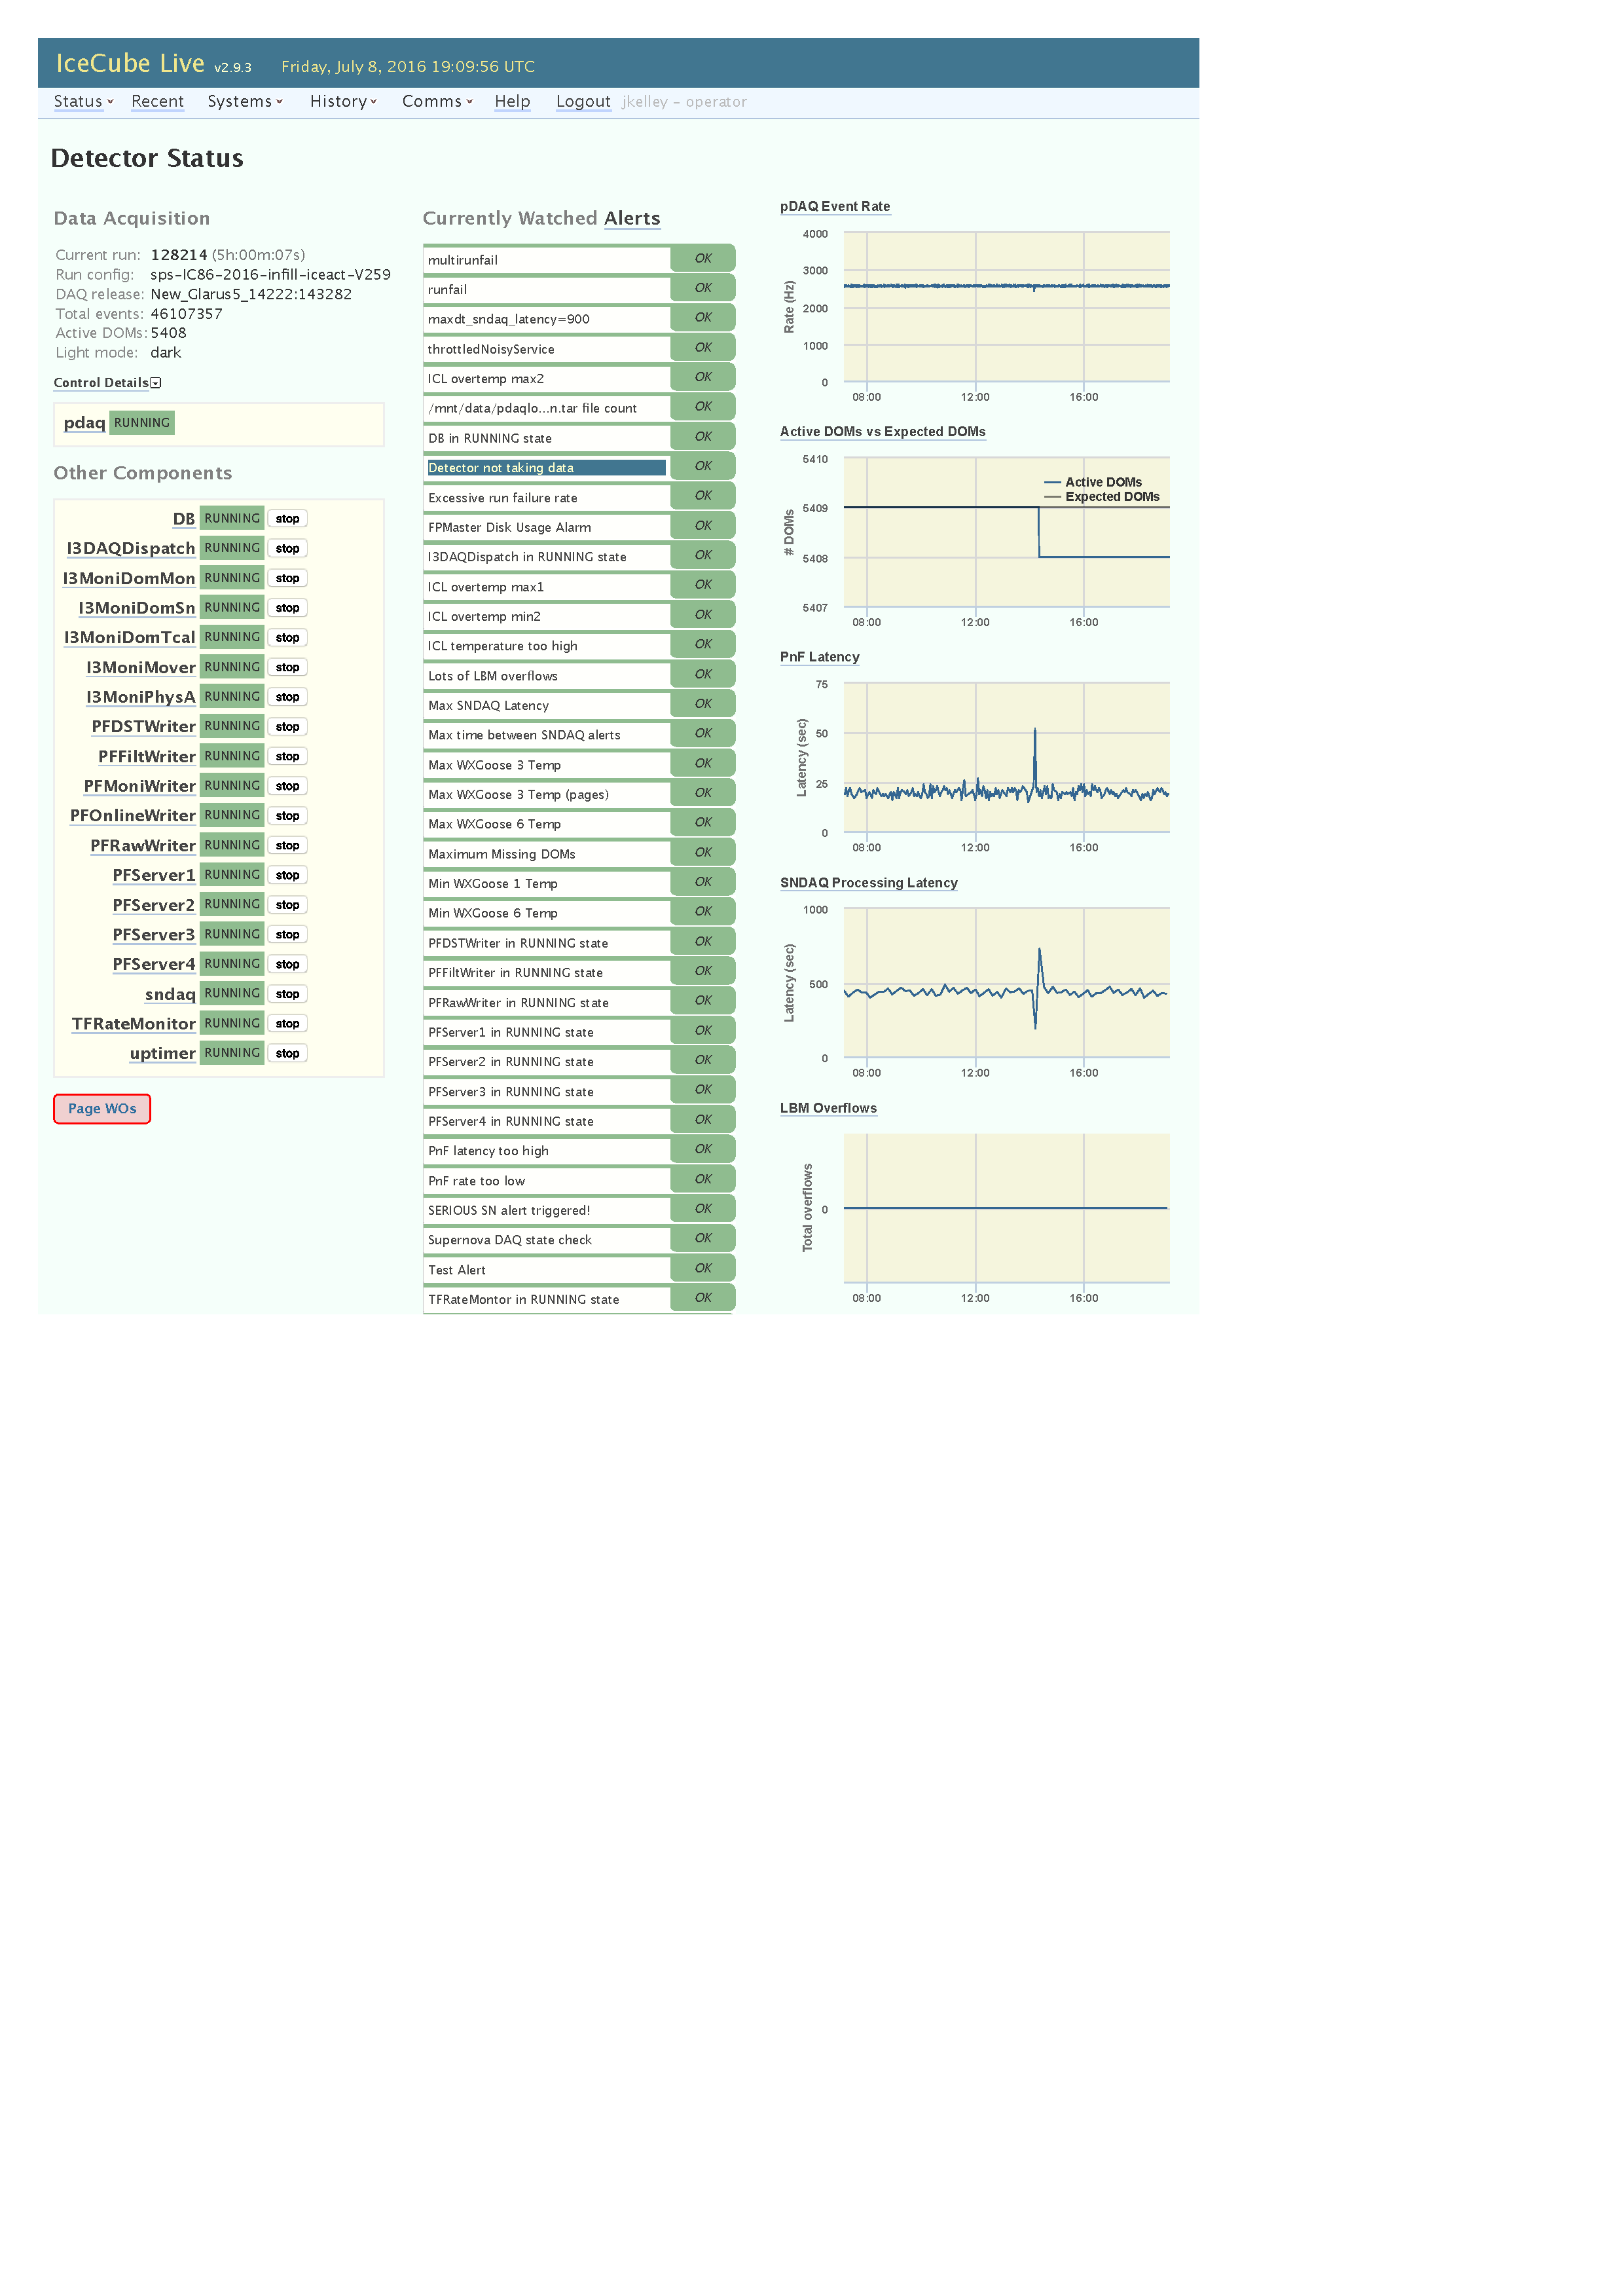
\includegraphics[width=1.0\textwidth]{graphics/online/live/live_screenshot_cropped.pdf}
 \caption{The IceCube Live website front page, showing near-realtime detector
   status.  One DOM has dropped out of data-taking in the run shown.  This
   ``operator'' view includes controls to start/stop components and to page
   the winterovers.} 
 \label{fig:live_screenshot}
\end{figure}

Finally, the IceCube Live website in the Northern Hemisphere can transmit
messages to LiveControl at SPS using the Iridium systems.  This capability
is used to link the commercial Slack chat service to a chat web page in
IceCube Live, allowing the IceCube winterover operators to communicate with
experts in the Northern Hemisphere during periods with no geosynchronous satellite
connectivity.  This connection also provides a limited capability to
control the detector, allowing operators in the Northern Hemisphere to
start/stop components or remotely issue HitSpool requests.

\subsection{\label{sec:operational_performance}Operational Performance}

Detector operational uptime is highly valued, in order to remain
sensitive to rare astrophysical transient events.  Many redundancies and
failsafes have been implemented, allowing an average detector uptime of greater
than 99\%. The detector uptime measures the fraction of total time
that some portion of the detector is taking data; sources of downtime
include the transitions between data-taking runs, power outages, and
DAQ interruptions due to software or hardware issues. All DOMHubs and servers are equipped with redundant power
supplies; these are in turn connected to redundant UPSes. This backup battery
power allows the detector to remain fully operational for about 15 minutes in the
event of a power outage.

Industry-standard Nagios monitoring software tracks the SPS hardware status and provides the link
between LiveControl and the paging system.  In the event of a hardware
or software failure that interrupts data-taking, a partial-detector configuration can
often be started automatically in parallel with the paging alert.
Within minutes, winterover operators start an optimal detector configuration
excluding only affected string(s), and then proceed to diagnose and fix the
issue.  Software issues can often be addressed via network access from the
South Pole Station, while hardware failures may require a visit to the ICL
for repairs (a 2-km walk).

The recovery of data from all but the last few minutes of runs that fail,
and the recent implementation of continuous data-taking, have improved
detector stability and decreased detector downtime. These features
contribute to an average ``clean uptime'' in recent years of 97--98\% of
full-detector, analysis-ready data, exceeding our target of 95\%.
Historical total detector uptime and clean uptime are shown in
Fig.~\ref{fig:clean-uptime}.   

\begin{figure}[!ht]
 \centering
 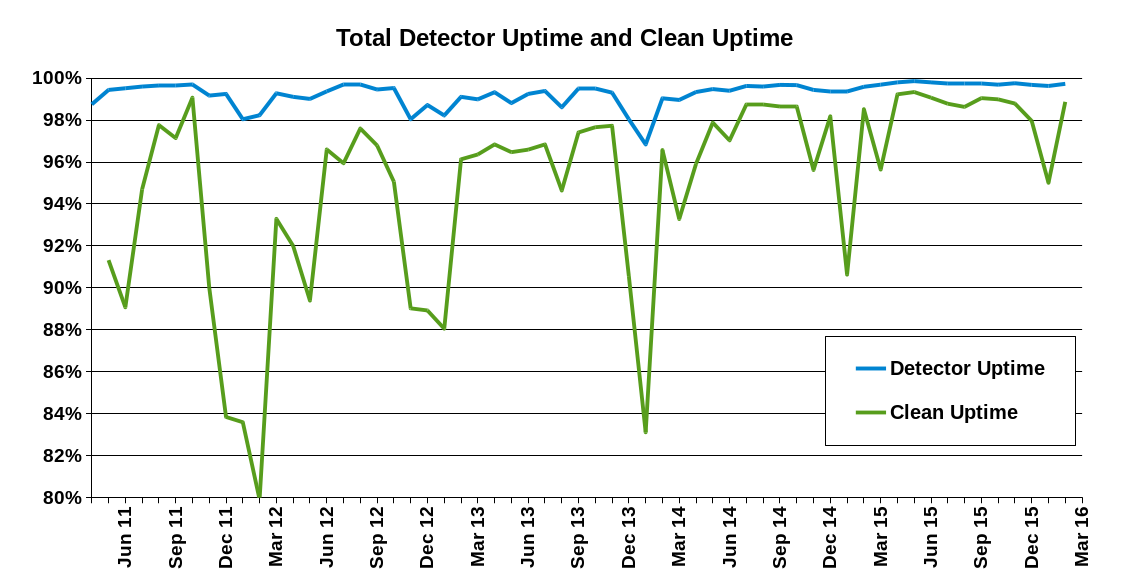
\includegraphics[width=1.0\textwidth]{graphics/uptime/clean-uptime.png}
 \caption{Detector uptime each month since the start of full-detector
   operation. ``Clean uptime'' indicates periods of analysis-ready,
   86-string data.} 
 \label{fig:clean-uptime}
\end{figure}

About 0.2\% of the loss in clean uptime is due to the failed portions of
runs that are not usable for analysis.  There is around 1\% of clean
uptime loss due to runs not using the full-detector configuration. This
occurs when certain components of the detector are excluded from the run
configuration during required repairs and maintenance; these
partial-detector runs are still useful for analyses that have less strict
requirements on the active detector volume or in the case of an exceptional
astrophysical transient event. There is approximately a 1\%
loss of clean uptime due to maintenance, commissioning, and verification
runs, and short runs that are less than 10 minutes in duration.  A
breakdown of total detector time by run period is shown in
Fig.~\ref{fig:period-performance}.  

\begin{figure}[!ht]
	\centering
    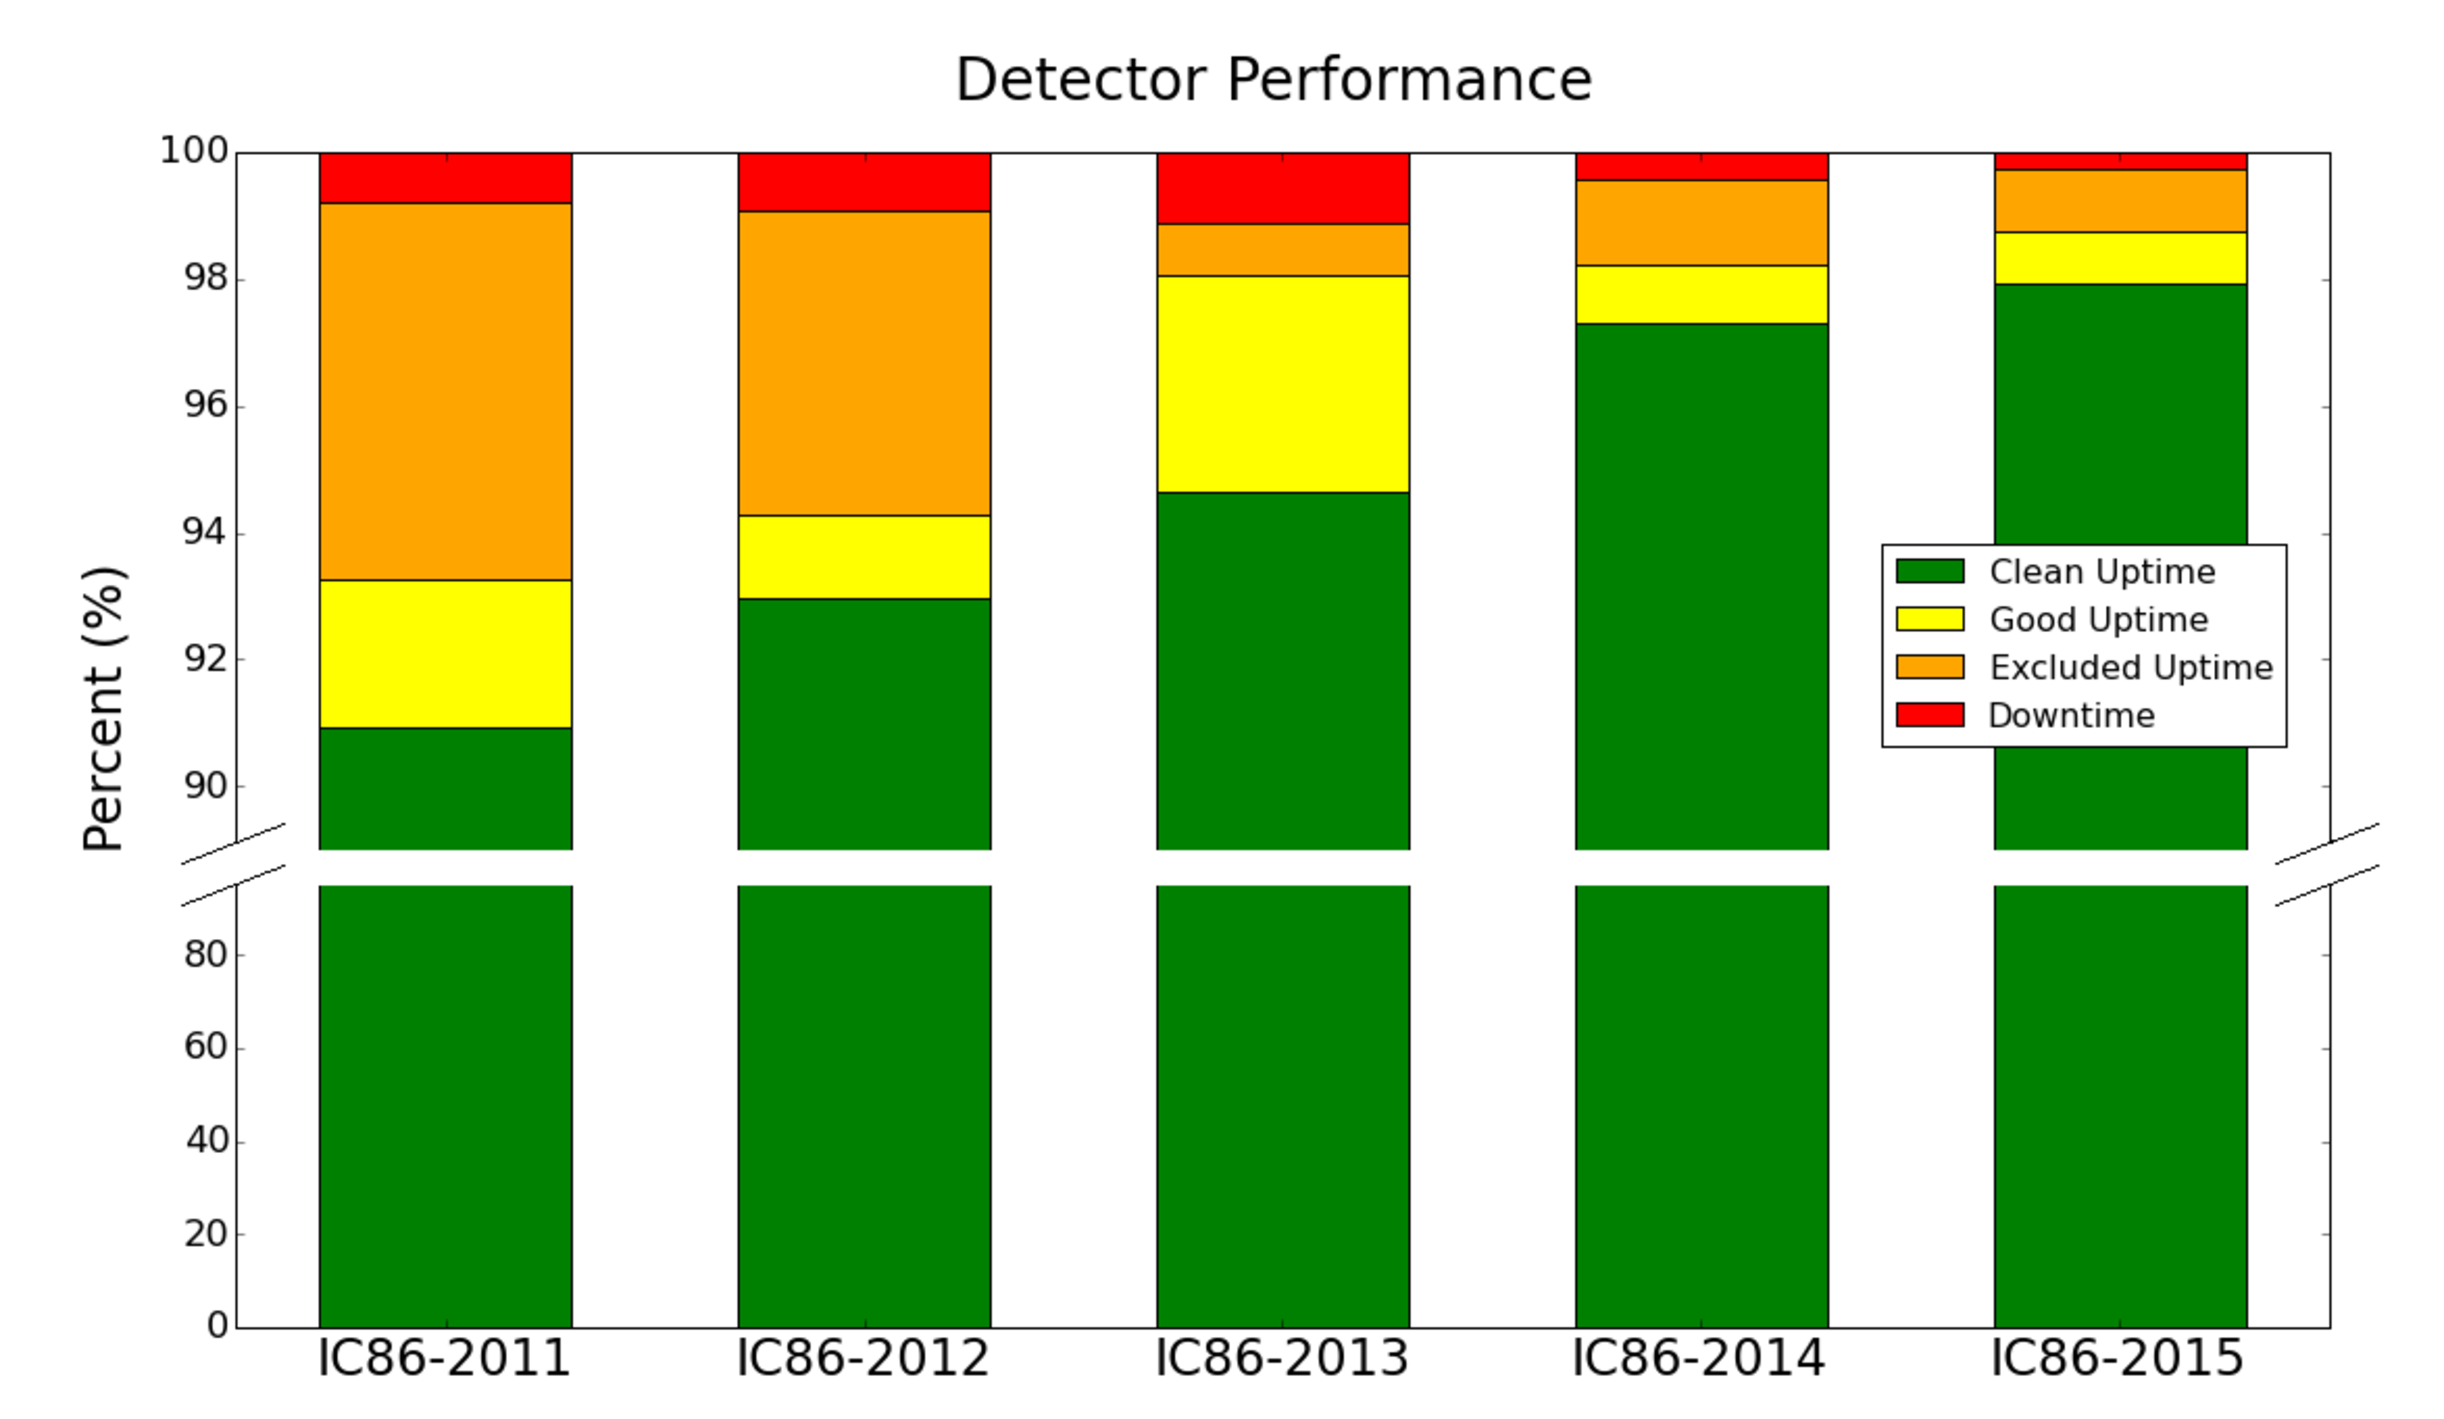
\includegraphics[width=0.8\textwidth]{graphics/uptime/bar-chart-broken-v2.pdf}
	\caption{Detector performance breakdown by
      run period.  Clean uptime indicates pristine, full-detector
      data; ``good uptime'' includes partial-detector runs that are
      otherwise healthy; and 
    ``excluded uptime'' indicates runs that are declared unusable for
      analysis.}
    \label{fig:period-performance}
\end{figure}


